% This LaTeX was auto-generated from MATLAB code.
% To make changes, update the MATLAB code and export to LaTeX again.

\documentclass{article}

\usepackage[utf8]{inputenc}
\usepackage[T1]{fontenc}
\usepackage{lmodern}
\usepackage{graphicx}
\usepackage{color}
\usepackage{listings}
\usepackage{hyperref}
\usepackage{amsmath}
\usepackage{amsfonts}
\usepackage{epstopdf}
\usepackage[table]{xcolor}
\usepackage{matlab}

\sloppy
\epstopdfsetup{outdir=./}
\graphicspath{ {./parametric_models_images/} }

\begin{document}

\matlabtitle{COMP0118 Coursework 1: Parametric Models}


\vspace{1em}
\matlabheading{1.1 Parameter Estimation and Mapping}


\vspace{1em}
\begin{par}
\begin{flushleft}
\textbf{Load and Inspect Data}
\end{flushleft}
\end{par}

\begin{par}
\begin{flushleft}
I first load the data from the file `data.mat`.
\end{flushleft}
\end{par}


\begin{matlabcode}
%loading data into matlab
load('data_p1/data.mat');
dwis = double(dwis);
dwis=permute(dwis, [4, 1, 2, 3]);
\end{matlabcode}

\begin{par}
\begin{flushleft}
I now display a single image slice to check that the image has been loaded correctly.
\end{flushleft}
\end{par}

\begin{matlabcode}
% middle slice of the 1st image volume, had b=0
imshow(flipud(squeeze(dwis(1, :, :, 72))'), []);
\end{matlabcode}
\begin{center}
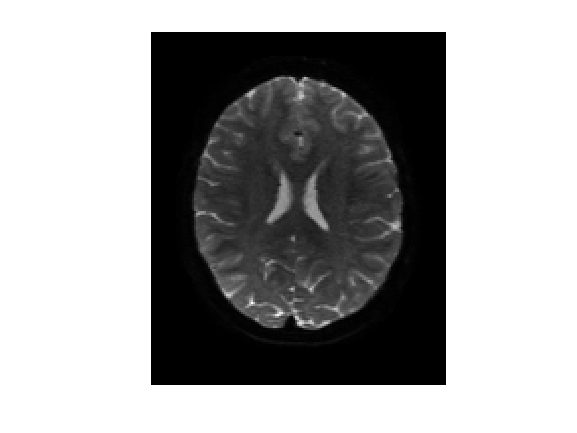
\includegraphics[width=\maxwidth{57.90265930757652em}]{figure_0.png}
\end{center}
\begin{matlabcode}
% Middle slice of the 2nd image volume, which has b=1000
imshow(flipud(squeeze(dwis(2,:,:,72))'), []);
\end{matlabcode}
\begin{center}
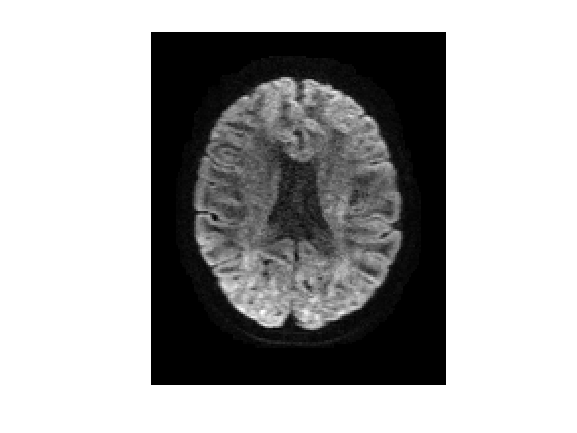
\includegraphics[width=\maxwidth{57.90265930757652em}]{figure_1.png}
\end{center}

\begin{par}
\begin{flushleft}
Next, I load the gradient directions stored in the file bvecs.
\end{flushleft}
\end{par}

\begin{matlabcode}
qhat = load('data_p1/bvecs');
% and the bvalue array
bvals = 1000*sum(qhat.*qhat);
\end{matlabcode}


\matlabheadingtwo{\textbf{Core Questions}}

\matlabheadingthree{\textbf{Q1.1.1 - Implementing linear diffusion tensor estimation and using it to map the mean diffusivity and fractional anisotropy over one slide of an image.}}


\vspace{1em}
\begin{par}
\begin{flushleft}
Perform fitting for a single voxel
\end{flushleft}
\end{par}


\begin{matlabcode}
% Select a single voxel
Avox = dwis(:, 92, 65, 72);

% Create the design matrix
G = [ones(1, 108); -bvals.*qhat(1, :).^2; -2*bvals.*qhat(1,:).*qhat(2,:); -2*bvals.*qhat(1,:).*qhat(3,:); -bvals.*qhat(2,:).^2; -2*bvals.*qhat(2,:).*qhat(3,:); -bvals.*qhat(3,:).^2]';

% Compute parameter vector x
x = G\log(Avox);
\end{matlabcode}


\begin{par}
\begin{flushleft}
Perform for all voxels
\end{flushleft}
\end{par}


\begin{matlabcode}
% Store diffusion tensor mapping here
dt_map72 = zeros(7, 145, 174);

% Precompute the design matrix
G = [ones(1, 108); -bvals.*qhat(1, :).^2; -2*bvals.*qhat(1,:).*qhat(2,:); -2*bvals.*qhat(1,:).*qhat(3,:); -bvals.*qhat(2,:).^2; -2*bvals.*qhat(2,:).*qhat(3,:); -bvals.*qhat(3,:).^2]';

% Repeat process for every voxel in slice
tic;
for i=1:145
    for j=1:174
        % Select voxel
        Avox = dwis(:, i, j, 72);
        
        if min(Avox) > 0
            % Compute x
            dt_map72(:, i, j) = G \ log(Avox);    
        end
    end
end
toc;

md_map72 = zeros(145, 174);
fa_map72 = zeros(145, 174);
cmap72 = zeros(145, 174, 3);

% Create the mean diffusivity map using dt_map72
for i=1:145
    for j=1:174
        
        % Select params for voxel
        x = dt_map72(:, i, j);
      
        % Get diffusion tensor
        D = [[x(2) x(3) x(4)]; [x(3) x(5) x(6)]; [x(4) x(6) x(7)]];
        
        % Compute eigenvectors and eigenvalues of D
        [V, L] = eig(D);
        Lbar = trace(L)/3;
        
        % Compute mean diffusivity
        md = (x(2, :) + x(5, :) + x(7, :)) / 3;
        md_map72(i, j) = md;
        
        % Compute fractional anisotropy map
        numerator = 0;
        denominator = 0;
        for k=1:3
            numerator = numerator + (L(k, k) - Lbar)^2;
            denominator = denominator + L(k, k)^2;
        end
        fa = sqrt((3/2) * numerator/denominator);
        fa_map72(i, j) = fa;
        
        % Find principal eigenvector
        [max_eigenval, idx] = max(diag(L));
        principal_e = V(:, idx);
        cmap72(i, j, :) = fa * abs(principal_e);
    end
end

% Visualize mean diffusion, fractional anisotropy and color maps
figure
imshow(flipud(md_map72'), [])
figure
imshow(flipud(fa_map72'), [])
figure
imshow(flipud(permute(cmap72, [2, 1, 3])), [])
\end{matlabcode}


\matlabheadingthree{\textbf{Q1.1.2 - Implement Ball-and-stick model to measure the density of axon fibres, indirectly, in each voxel.}}


\vspace{1em}
\begin{par}
\begin{flushleft}
First, I implement the Ball and stick model for a single voxel.
\end{flushleft}
\end{par}


\begin{matlabcode}
% Select a single voxel
Avox = dwis(:,92,65,72);

% Define a starting point for the non-linear fit
startx_noisy = [3.5e+00 3e-03 2.5e-01 0 0];

% Define various options for the non-linear fitting
% algorithm.
h=optimset('MaxFunEvals',20000,...
 'Algorithm','quasi-newton',...
 'TolX',1e-10,...
 'TolFun',1e-10);

% Now run the fitting
[parameter_hat,RESNORM,~,~]=fminunc('BallStickSSD',startx_noisy,h,Avox,bvals,qhat);

format short e
parameter_hat
RESNORM
\end{matlabcode}


\begin{par}
\begin{flushleft}
Now I implement the model on all voxels of the middle slice.
\end{flushleft}
\end{par}


\begin{matlabcode}
% Store fitted parameters for each voxel here
fitted_params_unconstrained_model = zeros(145, 174, 5);

tic;
for i=1:145
    for j=1:174
        % Select a single voxel
        Avox = dwis(:,i,j,72);

        if min(Avox) > 0
            % Define a starting point for the non-linear fit
            startx_noisy = [3.5e+00 3e-03 2.5e-01 0 0];
            
            % Define various options for the non-linear fitting
            % algorithm.
            h=optimset('MaxFunEvals',20000,...
             'Algorithm','quasi-newton',...
             'TolX',1e-10,...
             'TolFun',1e-10);
            
            % Now run the fitting
            [parameter_hat,RESNORM,~,~]=fminunc('BallStickSSD',startx_noisy,h,Avox,bvals,qhat);
         
            % Store parameter values in parameter_hat
            fitted_params_unconstrained_model(i, j, :) = parameter_hat;
        end
    end
end
toc;
\end{matlabcode}


\begin{par}
\begin{flushleft}
Evaluating the results by comparing the MRI signal predicted using the fitted parameter model result with the true signal values.
\end{flushleft}
\end{par}


\begin{matlabcode}
% Select results for the middle voxel
Avox = dwis(:, 92, 65, 72);
[S, SSD] = BallStickEval(fitted_params_unconstrained_model(92, 65, :), Avox, bvals, qhat);

% Plotted predicted values vs true values
figure
set(gcf, 'Position', [10, 10, 900, 500])
plot(Avox, ' bs', 'MarkerSize', 16, 'LineWidth', 4);
hold on;
plot(S, ' rx', 'MarkerSize', 16, 'LineWidth', 4);
xlabel('q index');
ylabel('S');
legend('Data','Model');
xlim([0,110]);
title(sprintf('Comparison of Model predicted signal S (red) and true measurement in Avox (blue) \nSSD = %.2f', SSD))
\end{matlabcode}


\matlabheadingthree{\textbf{Q1.1.3 - Adapt the implementation from 1.1.2 using the transformation method with }\texttt{\textbf{fminunc}}\textbf{ to allow for only realistic settings of parameters.}}


\vspace{1em}
\begin{par}
\begin{flushleft}
Implement on a single voxel
\end{flushleft}
\end{par}


\begin{matlabcode}
% Select a single voxel
Avox = dwis(:,92,65,72);

% Define a starting point for the non-linear fit
startx_noisy = [sqrt(3.5e+00) sqrt(3e-03) sqrt(-log(2.5e-01)) 0 0];

% Define various options for the non-linear fitting
% algorithm.
h=optimset('MaxFunEvals',20000,...
 'Algorithm','quasi-newton',...
 'TolX',1e-10,...
 'TolFun',1e-10);

% Now run the fitting
[parameter_hat,RESNORM,EXITFLAG,OUTPUT]=fminunc('BallStickSSD_transformation',startx_noisy,h,Avox,bvals,qhat);

% Transform parameters back to original values
parameter_hat(:, 1) = parameter_hat(:, 1)^2;
parameter_hat(:, 2) = parameter_hat(:, 2)^2;
parameter_hat(:, 3) = exp(-1 * parameter_hat(:, 3)^2);

format short e
parameter_hat
RESNORM
\end{matlabcode}


\begin{par}
\begin{flushleft}
Implement for all voxels
\end{flushleft}
\end{par}


\begin{matlabcode}
% Store fitted params for transformation model here
fitted_params_transformation_model = zeros(145, 174, 5);

tic;
for i=1:145
    for j=1:174
        % Select a single voxel
        Avox = dwis(:,i,j,72);
        
        if min(Avox) > 0
            % Define a starting point for the non-linear fit
            startx_noisy = [sqrt(3.5e+00) sqrt(3e-03) sqrt(-log(2.5e-01)) 0 0];
            
            % Define various options for the non-linear fitting
            % algorithm.
            h=optimset('MaxFunEvals',20000,...
             'Algorithm','quasi-newton',...
             'TolX',1e-10,...
             'TolFun',1e-10);
            
            % Now run the fitting
            [parameter_hat,RESNORM,EXITFLAG,OUTPUT]=fminunc('BallStickSSD_transformation',startx_noisy,h,Avox,bvals,qhat);
         
            % Transform parameters back to original values
            parameter_hat(:, 1) = parameter_hat(:, 1)^2;
            parameter_hat(:, 2) = parameter_hat(:, 2)^2;
            parameter_hat(:, 3) = exp(-1 * parameter_hat(:, 3)^2);
            
            % Store parameter values in parameter_hat
            fitted_params_transformation_model(i, j, :) = parameter_hat;
        end
    end
end
toc;
\end{matlabcode}


\begin{par}
\begin{flushleft}
Evaluating the results by comparing the MRI signal predicted using the fitted parameter model result with the true signal values.
\end{flushleft}
\end{par}


\begin{matlabcode}
% Select results for the middle voxel
Avox = dwis(:, 92, 65, 72);
[S, SSD] = BallStickEval(fitted_params_transformation_model(92, 65, :), Avox, bvals, qhat);

% Plotted predicted values vs true values
figure
set(gcf, 'Position', [10, 10, 900, 500])
plot(Avox, ' bs', 'MarkerSize', 16, 'LineWidth', 4);
hold on;
plot(S, ' rx', 'MarkerSize', 16, 'LineWidth', 4);
xlabel('q index');
ylabel('S');
legend('Data','Model');
xlim([0,110]);
title(sprintf('Comparison of Model predicted signal S (red) and true measurement in Avox (blue) \nSSD = %.2f', SSD))
\end{matlabcode}


\matlabheadingthree{\textbf{Q1.1.4 - Perform experiments now with many different starting points to assess if we really have converged to global minimum.}}


\begin{matlabcode}
n_runs = 100;
% Store errors per run here
errors_per_run = zeros(1, n_runs);

% Select a single voxel
i = 100;
j = 80;
Avox = dwis(:,i,j,72);

% Visualize where it is in the brain
figure
imshow(flipud(squeeze(dwis(1, :, :, 72))'), []);
axis on;
hold on;
plot(92, 65, 'r+', 'MarkerSize', 10, 'LineWidth', 2);
plot(72, 95, 'g+', 'MarkerSize', 10, 'LineWidth', 2);
plot(52, 88, 'b+', 'MarkerSize', 10, 'LineWidth', 2);
plot(100, 110, 'c+', 'MarkerSize', 10, 'LineWidth', 2);
plot(60, 50, 'm+', 'MarkerSize', 10, 'LineWidth', 2);
plot(72, 47, 'y+', 'MarkerSize', 10, 'LineWidth', 2);
plot(60, 120, 'w+', 'MarkerSize', 10, 'LineWidth', 2);
% plot(100, 80, 'w+', 'MarkerSize', 10, 'LineWidth', 2);

n = 1;
while n <= n_runs

    % Define a starting point for the non-linear fit
    startx = [3.5e+00 3e-03 2.5e-01 0 0];
    
    % Add gaussian noise to each of parameters
    startx_noisy(:, 1) = startx(:, 1) + 1e+03*randn;
    startx_noisy(:, 2) = startx(:, 2) + 1e-03*randn;
    while any(startx_noisy(:, 1:2) < 0)
        startx_noisy(:, 1) = startx(:, 1) + 1e+03*randn;
        startx_noisy(:, 2) = startx(:, 2) + 1e-03*randn;
    end
    startx_noisy(:, 3) = startx(:, 3) + 1e-01*randn;
    while startx_noisy(:, 3) > 1 || startx_noisy(:, 3) < 0
        startx_noisy(:, 3) = startx(:, 3) + 1e-01*randn;
    end
    startx_noisy(:, 4) = startx(:, 4) + 1e-01*randn;
    startx_noisy(:, 5) = startx(:, 5) + 1e-01*randn;
    
    % Perform inverse transformation on first three parameters
    startx_noisy(:, 1:2) = sqrt(startx_noisy(:, 1:2));
    startx_noisy(:, 3) = sqrt(-log(startx_noisy(:, 3)));
    
    % Define various options for the non-linear fitting
    % algorithm.
    h=optimset('MaxFunEvals',20000,...
     'Algorithm','quasi-newton',...
     'TolX',1e-10,...
     'TolFun',1e-10, 'Display', 'off');
    
    % Now run the fitting
    try
        [parameter_hat,RESNORM,EXITFLAG,OUTPUT]=fminunc('BallStickSSD_transformation',startx_noisy,h,Avox,bvals,qhat); 
    catch
        continue;
    end
    
    % Perform transformation back on parameters
    parameter_hat(:, 1) = parameter_hat(:, 1)^2;
    parameter_hat(:, 2) = parameter_hat(:, 2)^2;
    parameter_hat(:, 3) = exp(-parameter_hat(:, 3)^2);
    
    % Store
    errors_per_run(:, n) = RESNORM;
    
    n = n + 1;
end
\end{matlabcode}


\begin{par}
\begin{flushleft}
Plot the errors per run
\end{flushleft}
\end{par}


\begin{matlabcode}
figure
plot(n_runs)
hold on;
plot(errors_per_run)
xlabel('Iterations')
ylabel('Error')
title('Errors on every iteration')
\end{matlabcode}


\begin{matlabcode}
% Find proportion of trials with smallest value of RESNORM
min_error = min(errors_per_run)
count = 0;
tolerance = 0.1;
for n=1:n_runs
    if (errors_per_run(n) - min_error <= tolerance)
        count = count + 1;
    end
end

proportion = count / n_runs

% proportion = p(the run will find a global min) = p
% p(atleast 1 global min in n runs) = 1 - p(no global min in N runs)
% 0.95 = 1 - nC0*p^0*(1-p)^n
n_runs = log(0.05)/log(1-proportion)
\end{matlabcode}


\matlabheadingthree{Q1.1.5 - Create parameter maps over image slice for S0, d, f and RESNORM. Also Create a fibre direction map.}


\begin{matlabcode}
% Select 72nd image slice
image = dwis(:, :, :, 72);

% Compute feature maps for this slice
parameter_maps = createParameterMaps(image, bvals, qhat, 10);
\end{matlabcode}


\begin{matlabcode}
% Select parameter maps
S0_map72 = parameter_maps(:, :, 1);
d_map72 = parameter_maps(:, :, 2);
f_map72 = parameter_maps(:, :, 3);
theta_map72 = parameter_maps(:, :, 4);
phi_map72 = parameter_maps(:, :, 5);
RESNORM_map72 = parameter_maps(:, :, 6);

% Visualize the feature maps
figure
imshow(flipud(S0_map72'), [])

figure
imshow(flipud(d_map72'), [])

figure
imshow(flipud(f_map72'), [])

figure
imshow(flipud(RESNORM_map72'), [])

% compute fibre direction map
figure
set(gcf, 'Position', [10, 10, 450, 500])
fibredir_map72 = zeros(145, 174, 2);
for i=1:145
    for j=1:174
        fibredir_map72(i, j, :) = f_map72(i, j) .* [cos(theta_map72(i, j))*sin(theta_map72(i, j)) sin(phi_map72(i, j))*sin(theta_map72(i, j))];
    end
end
quiver(flipud(fibredir_map72(:, :, 1)'), flipud(fibredir_map72(:, :, 2)'))
\end{matlabcode}
\begin{matlaboutput}
Unrecognized function or variable 'finBestFit'.

Error in generateDataSet (line 14)
            [parameter_hat, ~] = finBestFit(3, Avox, bvals, qhat);
Warning: NEWFF used in an obsolete way.
          See help for NEWFF to update calls to the new argument list.
 
net =

    Neural Network
 
              name: 'Custom Neural Network'
          userdata: (your custom info)
 
    dimensions:
 
         numInputs: 1
         numLayers: 2
        numOutputs: 1
    numInputDelays: 0
    numLayerDelays: 0
 numFeedbackDelays: 0
 numWeightElements: 1145
        sampleTime: 1
 
    connections:
 
       biasConnect: [1; 1]
      inputConnect: [1; 0]
      layerConnect: [0 0; 1 0]
     outputConnect: [0 1]
 
    subobjects:
 
             input: Equivalent to inputs{1}
            output: Equivalent to outputs{2}
 
            inputs: {1x1 cell array of 1 input}
            layers: {2x1 cell array of 2 layers}
           outputs: {1x2 cell array of 1 output}
            biases: {2x1 cell array of 2 biases}
      inputWeights: {2x1 cell array of 1 weight}
      layerWeights: {2x2 cell array of 1 weight}
 
    functions:
 
          adaptFcn: 'adaptwb'
        adaptParam: (none)
          derivFcn: 'defaultderiv'
         divideFcn: (none)
       divideParam: (none)
        divideMode: 'sample'
           initFcn: 'initlay'
        performFcn: 'mse'
      performParam: .regularization, .normalization
          plotFcns: {'plotperform', 'plottrainstate',
                    'plotregression'}
        plotParams: {1x3 cell array of 3 params}
          trainFcn: 'trainlm'
        trainParam: .showWindow, .showCommandLine, .show, .epochs,
                    .time, .goal, .min_grad, .max_fail, .mu, .mu_dec,
                    .mu_inc, .mu_max, .lr
 
    weight and bias values:
 
                IW: {2x1 cell} containing 1 input weight matrix
                LW: {2x2 cell} containing 1 layer weight matrix
                 b: {2x1 cell} containing 2 bias vectors
 
    methods:
 
             adapt: Learn while in continuous use
         configure: Configure inputs & outputs
            gensim: Generate Simulink model
              init: Initialize weights & biases
           perform: Calculate performance
               sim: Evaluate network outputs given inputs
             train: Train network with examples
              view: View diagram
       unconfigure: Unconfigure inputs & outputs
 
\end{matlaboutput}
\begin{center}
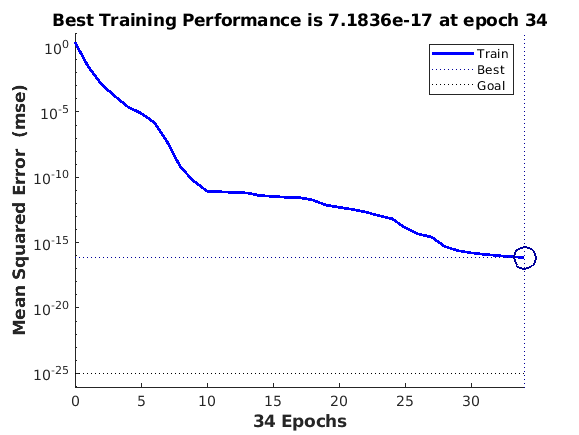
\includegraphics[width=\maxwidth{57.90265930757652em}]{figure_2.png}
\end{center}
\begin{matlaboutput}
net =

    Neural Network
 
              name: 'Custom Neural Network'
          userdata: (your custom info)
 
    dimensions:
 
         numInputs: 1
         numLayers: 2
        numOutputs: 1
    numInputDelays: 0
    numLayerDelays: 0
 numFeedbackDelays: 0
 numWeightElements: 1145
        sampleTime: 1
 
    connections:
 
       biasConnect: [1; 1]
      inputConnect: [1; 0]
      layerConnect: [0 0; 1 0]
     outputConnect: [0 1]
 
    subobjects:
 
             input: Equivalent to inputs{1}
            output: Equivalent to outputs{2}
 
            inputs: {1x1 cell array of 1 input}
            layers: {2x1 cell array of 2 layers}
           outputs: {1x2 cell array of 1 output}
            biases: {2x1 cell array of 2 biases}
      inputWeights: {2x1 cell array of 1 weight}
      layerWeights: {2x2 cell array of 1 weight}
 
    functions:
 
          adaptFcn: 'adaptwb'
        adaptParam: (none)
          derivFcn: 'defaultderiv'
         divideFcn: (none)
       divideParam: (none)
        divideMode: 'sample'
           initFcn: 'initlay'
        performFcn: 'mse'
      performParam: .regularization, .normalization
          plotFcns: {'plotperform', 'plottrainstate',
                    'plotregression'}
        plotParams: {1x3 cell array of 3 params}
          trainFcn: 'trainlm'
        trainParam: .showWindow, .showCommandLine, .show, .epochs,
                    .time, .goal, .min_grad, .max_fail, .mu, .mu_dec,
                    .mu_inc, .mu_max, .lr
 
    weight and bias values:
 
                IW: {2x1 cell} containing 1 input weight matrix
                LW: {2x2 cell} containing 1 layer weight matrix
                 b: {2x1 cell} containing 2 bias vectors
 
    methods:
 
             adapt: Learn while in continuous use
         configure: Configure inputs & outputs
            gensim: Generate Simulink model
              init: Initialize weights & biases
           perform: Calculate performance
               sim: Evaluate network outputs given inputs
             train: Train network with examples
              view: View diagram
       unconfigure: Unconfigure inputs & outputs
 
y = 5x1    
1.0e+-10 *

   -0.1387
   -0.3083
    0.3747
    0.0654
   -0.4293

ans = 5x1    
     0
     0
     0
     0
     0

Error using bsxfun
Non-singleton dimensions of the two input arrays must match each other.

Error in gsubtract>calc_general (line 40)
    c = bsxfun(@minus,a,b);

Error in gsubtract>calc_cell (line 60)
  for i=1:numel(a), c{i} = calc_general(a{i},b); end

Error in gsubtract (line 24)
  c = calc_cell(a,b);

Error in nncalc.perform (line 17)
e = gsubtract(t,y);

Error in network/perform (line 33)
perf = nncalc.perform(net,t,y,ew,net.performParam);
\end{matlaboutput}


\begin{matlabcode}
[trainX, trainY] = generateDataSet(dwis, bvals, qhat);
\end{matlabcode}
\begin{matlaboutput}
Run 1
Run 2
Run 2
Run 2
Run 2
Run 3
Run 1
Run 2
Run 3
Run 3
Run 3
Run 3
Run 1
Run 1
Run 2
Run 2
Run 2
Run 3
Run 1
Run 1
Run 2
Run 3
Run 3
Run 3
Run 1
Run 2
Run 2
Run 2
Run 3
Run 1
Run 1
Run 2
Run 2
Run 2
Run 3
Run 3
Run 1
Run 1
Run 2
Run 2
Run 3
Run 1
Run 2
Run 2
Run 2
Run 2
Run 2
Run 3
Run 3
Run 3
Run 3
Run 3
Run 3
Run 1
Run 1
Run 2
Run 2
Run 3
Run 1
Run 1
Run 1
Run 2
Run 2
Run 3
Run 3
Run 3
Run 1
Run 1
Run 1
Run 1
Run 2
Run 3
Run 3
Run 3
Run 1
Run 1
Run 1
Run 2
Run 3
Run 3
Run 3
Run 1
Run 2
Run 3
Run 1
Run 1
Run 2
Run 3
Run 3
Run 1
Run 2
Run 2
Run 2
Run 2
Run 2
Run 2
Run 3
Run 1
Run 1
Run 1
Run 1
Run 1
Run 2
Run 2
Run 3
Run 3
Run 1
Run 2
Run 2
Run 3
Run 1
Run 1
Run 1
Run 1
Run 2
Run 3
Run 3
Run 1
Run 1
Run 1
Run 2
Run 3
Run 3
Run 1
Run 2
Run 3
Run 3
Run 1
Run 1
Run 1
Run 2
Run 2
Run 2
Run 3
Run 1
Run 2
Run 3
Run 3
Run 3
Run 1
Run 1
Run 2
Run 3
Run 3
Run 1
Run 2
Run 2
Run 2
Run 2
Run 2
Run 3
Run 1
Run 1
Run 2
Run 3
Run 3
Run 3
Run 1
Run 2
Run 2
Run 3
Run 1
Run 2
Run 3
Run 1
Run 1
Run 1
Run 2
Run 3
Run 1
Run 1
Run 1
Run 1
Run 1
Run 1
Run 1
Run 1
Run 2
Run 2
Run 2
Run 2
Run 3
Run 3
Run 1
Run 1
Run 2
Run 3
Run 3
Run 1
Run 2
Run 3
Run 3
Run 1
Run 1
Run 2
Run 2
Run 3
Run 3
Run 1
Run 1
Run 2
Run 3
Run 3
Run 3
Run 1
Run 2
Run 3
Run 1
Run 2
Run 3
Run 3
Run 1
Run 1
Run 2
Run 3
Run 1
Run 1
Run 2
Run 3
Run 3
Run 1
Run 1
Run 2
Run 2
Run 2
Run 3
Run 1
Run 2
Run 3
Run 3
Run 3
Run 3
Run 1
Run 1
Run 1
Run 2
Run 3
Run 1
Run 1
Run 2
Run 2
Run 3
Run 3
Run 1
Run 1
Run 2
Run 3
Run 3
Run 3
Run 1
Run 2
Run 3
Run 1
Run 2
Run 3
Run 3
Run 3
Run 1
Run 2
Run 2
Run 2
Run 2
Run 2
Run 3
Run 1
Run 1
Run 2
Run 3
Run 3
Run 3
Run 1
Run 1
Run 2
Run 3
Run 1
Run 1
Run 2
Run 3
Run 3
Run 3
Run 3
Run 3
Run 1
Run 2
Run 3
Run 1
Run 1
Run 2
Run 3
Run 1
Run 1
Run 1
Run 1
Run 1
Run 1
Run 1
Run 1
Run 1
Run 2
Run 3
Run 3
Run 3
Run 3
Run 1
Run 2
Run 3
Run 3
Run 3
Run 3
Run 3
Run 1
Run 2
Run 3
Run 1
Run 2
Run 3
Run 1
Run 2
Run 3
Run 1
Run 1
Run 1
Run 2
Run 3
Run 1
Run 1
Run 2
Run 2
Run 2
Run 3
Run 3
Run 1
Run 2
Run 3
Run 3
Run 3
Run 3
Run 3
Run 1
Run 1
Run 1
Run 1
Run 1
Run 1
Run 2
Run 2
Run 2
Run 3
Run 3
Run 1
Run 2
Run 3
Run 3
Run 1
Run 2
Run 2
Run 2
Run 2
Run 2
Run 2
Run 2
Run 2
Run 2
Run 2
Run 3
Run 1
Run 1
Run 2
Run 3
Run 1
Run 2
Run 2
Run 3
Run 1
Run 2
Run 3
Run 3
Run 3
Run 1
Run 2
Run 3
Run 1
Run 1
Run 2
Run 3
Run 3
Run 1
Run 2
Run 3
Run 3
Run 1
Run 1
Run 1
Run 1
Run 2
Run 3
Run 1
Run 1
Run 2
Run 2
Run 3
Run 1
Run 2
Run 3
Run 3
Run 3
Run 3
Run 1
Run 2
Run 3
Run 3
Run 1
Run 2
Run 3
Run 1
Run 1
Run 1
Run 1
Run 2
Run 2
Run 3
Run 3
Run 1
Run 1
Run 1
Run 1
Run 2
Run 2
Run 3
Run 1
Run 1
Run 1
Run 1
Run 1
Run 1
Run 1
Run 1
Run 1
Run 2
Run 2
Run 3
Run 1
Run 2
Run 2
Run 3
Run 1
Run 2
Run 3
Run 3
Run 3
Run 1
Run 1
Run 1
Run 1
Run 1
Run 1
Run 1
Run 2
Run 3
Run 1
Run 1
Run 1
Run 2
Run 2
Run 3
Run 1
Run 1
Run 2
Run 3
Run 3
Run 1
Run 1
Run 1
Run 1
Run 2
Run 2
Run 3
Run 3
Run 1
Run 1
Run 1
Run 2
Run 3
Run 1
Run 1
Run 1
Run 1
Run 1
Run 1
Run 1
Run 2
Run 2
Run 3
Run 3
Run 1
Run 1
Run 1
Run 1
Run 1
Run 2
Run 3
Run 3
Run 3
Run 1
Run 1
Run 1
Run 1
Run 2
Run 3
Run 1
Run 1
Run 2
Run 3
Run 1
Run 2
Run 3
Run 3
Run 3
Run 3
Run 3
Run 1
Run 2
Run 3
Run 3
Run 3
Run 3
Run 1
Run 2
Run 2
Run 3
Run 1
Run 2
Run 2
Run 2
Run 2
Run 3
Run 3
Run 3
Run 1
Run 2
Run 2
Run 3
Run 3
Run 3
Run 3
Run 1
Run 2
Run 2
Run 3
Run 3
Run 3
Run 3
Run 1
Run 2
Run 3
Run 3
Run 1
Run 2
Run 2
Run 3
Run 3
Run 3
Run 3
Run 3
Run 1
Run 1
Run 1
Run 2
Run 3
Run 3
Run 3
Run 1
Run 2
Run 3
Run 1
Run 2
Run 2
Run 3
Run 3
Run 3
Run 3
Run 3
Run 1
Run 1
Run 1
Run 2
Run 2
Run 2
Run 3
Run 3
Run 3
Run 3
Run 1
Run 1
Run 2
Run 3
Run 3
Run 3
Run 1
Run 1
Run 1
Run 2
Run 2
Run 2
Run 2
Run 2
Run 3
Run 1
Run 1
Run 1
Run 1
Run 2
Run 2
Run 3
Run 1
Run 2
Run 2
Run 2
Run 2
Run 3
Run 3
Run 3
Run 3
Run 1
Run 2
Run 2
Run 2
Run 2
Run 3
Run 3
Run 3
Run 1
Run 2
Run 2
Run 2
Run 3
Run 3
Run 1
Run 1
Run 2
Run 3
Run 1
Run 1
Run 1
Run 2
Run 3
Run 3
Run 1
Run 2
Run 2
Run 2
Run 3
Run 3
Run 1
Run 1
Run 2
Run 2
Run 2
Run 3
Run 3
Run 3
Run 3
Run 1
Run 1
Run 2
Run 3
Run 1
Run 2
Run 3
Run 3
Run 3
Run 1
Run 1
Run 2
Run 3
Run 3
Run 3
Run 3
Run 1
Run 1
Run 1
Run 1
Run 1
Run 1
Run 2
Run 3
Run 1
Run 2
Run 2
Run 2
Run 3
Run 3
Run 3
Run 1
Run 2
Run 3
Run 3
Run 1
Run 2
Run 3
Run 3
Run 3
Run 3
Run 3
Run 1
Run 1
Run 1
Run 1
Run 1
Run 1
Run 1
Run 2
Run 2
Run 3
Run 1
Run 1
Run 1
Run 2
Run 3
Run 1
Run 1
Run 2
Run 2
Run 2
Run 3
Run 1
Run 2
Run 2
Run 2
Run 3
Run 3
Run 3
Run 3
Run 1
Run 2
Run 2
Run 2
Run 2
Run 2
Run 3
Run 1
Run 1
Run 2
Run 3
Run 1
Run 1
Run 1
Run 1
Run 1
Run 2
Run 3
Run 3
Run 1
Run 2
Run 3
Run 1
Run 2
Run 3
Run 1
Run 2
Run 2
Run 2
Run 3
Run 1
Run 2
Run 3
Run 3
Run 3
Run 3
Run 1
Run 1
Run 2
Run 3
Run 3
Run 1
Run 2
Run 3
Run 3
Run 1
Run 1
Run 2
Run 2
Run 3
Run 1
Run 1
Run 2
Run 3
Run 3
Run 3
Run 3
Run 1
Run 1
Run 2
Run 3
Run 1
Run 2
Run 2
Run 2
Run 3
Run 3
Run 3
Run 1
Run 2
Run 2
Run 2
Run 3
Run 3
Run 3
Run 3
Run 1
Run 1
Run 1
Run 2
Run 3
Run 1
Run 2
Run 2
Run 3
Run 1
Run 2
Run 2
Run 2
Run 2
Run 3
Run 3
Run 1
Run 1
Run 2
Run 2
Run 2
Run 3
Run 1
Run 2
Run 2
Run 2
Run 3
Run 1
Run 1
Run 1
Run 1
Run 2
Run 2
Run 2
Run 2
Run 3
Run 3
Run 1
Run 1
Run 1
Run 2
Run 3
Run 1
Run 1
Run 1
Run 1
Run 1
Run 1
Run 2
Run 2
Run 3
Run 1
Run 2
Run 3
Run 1
Run 1
Run 2
Run 2
Run 2
Run 3
Run 1
Run 2
Run 2
Run 3
Run 1
Run 1
Run 2
Run 2
Run 3
Run 1
Run 2
Run 3
Run 3
Run 3
Run 1
Run 1
Run 2
Run 2
Run 2
Run 2
Run 3
Run 1
Run 2
Run 2
Run 3
Run 3
Run 1
Run 1
Run 2
Run 3
Run 1
Run 1
Run 2
Run 3
Run 1
Run 2
Run 2
Run 2
Run 3
Run 3
Run 1
Run 1
Run 1
Run 2
Run 3
Run 3
Run 1
Run 1
Run 2
Run 2
Run 2
Run 2
Run 2
Run 2
Run 3
Run 1
Run 1
Run 1
Run 1
Run 2
Run 2
Run 3
Run 3
Run 3
Run 1
Run 2
Run 2
Run 3
Run 3
Run 1
Run 1
Run 1
Run 2
Run 2
Run 3
Run 3
Run 1
Run 1
Run 1
Run 2
Run 3
Run 3
Run 3
Run 1
Run 2
Run 2
Run 2
Run 2
Run 3
Run 1
Run 1
Run 2
Run 2
Run 2
Run 2
Run 3
Run 3
Run 3
Run 1
Run 2
Run 2
Run 2
Run 3
Run 1
Run 1
Run 1
Run 2
Run 2
Run 3
Run 1
Run 1
Run 1
Run 2
Run 2
Run 3
Run 3
Run 1
Run 2
Run 2
Run 3
Run 1
Run 1
Run 2
Run 3
Run 1
Run 1
Run 1
Run 1
Run 2
Run 2
Run 3
Run 1
Run 1
Run 2
Run 2
Run 3
Run 1
Run 2
Run 2
Run 3
Run 3
Run 1
Run 2
Run 3
Run 1
Run 2
Run 2
Run 3
Run 3
Run 3
Run 1
Run 2
Run 2
Run 2
Run 3
Run 3
Run 3
Run 1
Run 2
Run 3
Run 3
Run 1
Run 1
Run 1
Run 1
Run 1
Run 1
Run 1
Run 2
Run 3
Run 3
Run 3
Run 3
Run 3
Run 3
Run 3
Run 3
Run 1
Run 1
Run 1
Run 2
Run 2
Run 3
Run 3
Run 1
Run 2
Run 3
Run 1
Run 1
Run 1
Run 1
Run 1
Run 2
Run 2
Run 2
Run 2
Run 2
Run 3
Run 3
Run 3
Run 1
Run 2
Run 3
Run 3
Run 3
Run 3
Run 3
Run 3
Run 3
Run 1
Run 1
Run 2
Run 2
Run 2
Run 3
Run 1
Run 2
Run 2
Run 3
Run 1
Run 2
Run 3
Run 1
Run 2
Run 2
Run 3
Run 1
Run 2
Run 2
Run 3
Run 1
Run 2
Run 2
Run 3
Run 3
Run 3
Run 1
Run 2
Run 2
Run 2
Run 3
Run 3
Run 3
Run 3
Run 3
Run 1
Run 1
Run 2
Run 2
Run 3
Run 1
Run 2
Run 3
Run 3
Run 3
Run 1
Run 1
Run 1
Run 2
Run 2
Run 2
Run 3
Run 1
Run 1
Run 1
Run 2
Run 2
Run 3
Run 3
Run 3
Run 3
Run 1
Run 1
Run 1
Run 2
Run 3
Run 1
Run 2
Run 2
Run 3
Run 1
Run 1
Run 2
Run 2
Run 3
Run 1
Run 1
Run 2
Run 3
Run 3
Run 3
Run 3
Run 1
Run 1
Run 1
Run 1
Run 2
Run 3
Run 1
Run 1
Run 1
Run 2
Run 2
Run 2
Run 2
Run 3
Run 3
Run 1
Run 2
Run 3
Run 3
Run 3
Run 1
Run 1
Run 2
Run 2
Run 2
Run 2
Run 3
Run 3
Run 1
Run 2
Run 2
Run 2
Run 2
Run 3
Run 1
Run 2
Run 3
Run 3
Run 1
Run 1
Run 1
Run 2
Run 3
Run 3
Run 3
Run 1
Run 1
Run 2
Run 3
Run 1
Run 2
Run 3
Run 1
Run 1
Run 1
Run 2
Run 3
Run 1
Run 2
Run 2
Run 2
Run 3
Run 3
Run 1
Run 2
Run 3
Run 3
Run 3
Run 1
Run 2
Run 3
Run 1
Run 1
Run 1
Run 2
Run 3
Run 3
Run 1
Run 1
Run 1
Run 2
Run 2
Run 3
Run 1
Run 2
Run 3
Run 3
Run 1
Run 1
Run 1
Run 2
Run 3
Run 3
Run 3
Run 3
Run 1
Run 1
Run 1
Run 2
Run 3
Run 1
Run 1
Run 1
Run 2
Run 2
Run 3
Run 3
Run 3
Run 3
Run 1
Run 1
Run 2
Run 2
Run 2
Run 3
Run 1
Run 2
Run 3
Run 3
Run 3
Run 1
Run 1
Run 2
Run 2
Run 2
Run 2
Run 3
Run 3
Run 1
Run 1
Run 2
Run 2
Run 3
Run 3
Run 1
Run 2
Run 3
Run 3
Run 1
Run 2
Run 2
Run 3
Run 1
Run 2
Run 3
Run 1
Run 2
Run 2
Run 3
Run 1
Run 2
Run 3
Run 1
Run 1
Run 1
Run 1
Run 1
Run 1
Run 2
Run 2
Run 2
Run 3
Run 3
Run 3
Run 3
Run 3
Run 3
Run 1
Run 1
Run 1
Run 2
Run 3
Run 1
Run 2
Run 3
Run 3
Run 3
Run 1
Run 2
Run 2
Run 2
Run 2
Run 3
Run 3
Run 3
Run 1
Run 2
Run 2
Run 3
Run 1
Run 2
Run 3
Run 3
Run 1
Run 2
Run 3
Run 1
Run 1
Run 2
Run 3
Run 3
Run 3
Run 1
Run 2
Run 2
Run 3
Run 1
Run 1
Run 1
Run 2
Run 2
Run 3
Run 3
Run 1
Run 2
Run 2
Run 3
Run 1
Run 2
Run 2
Run 3
Run 1
Run 2
Run 3
Run 1
Run 1
Run 1
Run 1
Run 2
Run 3
Run 1
Run 1
Run 2
Run 3
Run 3
Run 3
Run 3
Run 1
Run 1
Run 1
Run 1
Run 2
Run 3
Run 3
Run 1
Run 1
Run 2
Run 3
Run 1
Run 1
Run 1
Run 2
Run 2
Run 3
Run 3
Run 3
Run 3
Run 1
Run 1
Run 1
Run 1
Run 1
Run 1
Run 2
Run 2
Run 2
Run 2
Run 2
Run 2
Run 3
Run 3
Run 3
Run 1
Run 1
Run 1
Run 1
Run 2
Run 3
Run 3
Run 3
Run 1
Run 2
Run 2
Run 2
Run 2
Run 3
Run 1
Run 2
Run 3
Run 3
Run 1
Run 1
Run 2
Run 2
Run 2
Run 3
Run 3
Run 1
Run 2
Run 2
Run 3
Run 3
Run 3
Run 3
Run 1
Run 1
Run 1
Run 2
Run 2
Run 3
Run 3
Run 3
Run 1
Run 2
Run 3
Run 3
Run 1
Run 2
Run 2
Run 3
Run 1
Run 1
Run 2
Run 3
Run 3
Run 3
Run 1
Run 1
Run 2
Run 3
Run 3
Run 1
Run 2
Run 3
Run 1
Run 1
Run 2
Run 2
Run 3
Run 1
Run 1
Run 2
Run 2
Run 3
Run 1
Run 1
Run 2
Run 3
Run 1
Run 1
Run 1
Run 1
Run 1
Run 1
Run 2
Run 3
Run 1
Run 2
Run 2
Run 2
Run 2
Run 3
Run 1
Run 1
Run 1
Run 2
Run 2
Run 3
Run 3
Run 1
Run 1
Run 2
Run 3
Run 3
Run 3
Run 1
Run 2
Run 3
Run 3
Run 3
Run 1
Run 1
Run 1
Run 2
Run 2
Run 3
Run 3
Run 3
Run 1
Run 2
Run 3
Run 1
Run 1
Run 1
Run 2
Run 2
Run 2
Run 2
Run 2
Run 2
Run 2
Run 3
Run 1
Run 1
Run 2
Run 2
Run 3
Run 1
Run 1
Run 2
Run 3
Run 1
Run 2
Run 3
Run 1
Run 1
Run 1
Run 1
Run 2
Run 3
Run 3
Run 1
Run 2
Run 3
Run 1
Run 2
Run 3
Run 1
Run 1
Run 2
Run 3
Run 3
Run 1
Run 2
Run 3
Run 3
Run 3
Run 3
Run 1
Run 1
Run 1
Run 1
Run 1
Run 2
Run 2
Run 2
Run 3
Run 1
Run 2
Run 3
Run 1
Run 1
Run 1
Run 2
Run 3
Run 3
Run 1
Run 2
Run 3
Run 1
Run 2
Run 3
Run 1
Run 1
Run 1
Run 1
Run 1
Run 1
Run 2
Run 2
Run 2
Run 2
Run 3
Run 1
Run 2
Run 3
Run 3
Run 3
Run 3
Run 3
Run 1
Run 1
Run 1
Run 1
Run 1
Run 2
Run 3
Run 1
Run 2
Run 2
Run 3
Run 1
Run 2
Run 2
Run 2
Run 3
Run 3
Run 1
Run 2
Run 2
Run 3
Run 1
Run 1
Run 1
Run 2
Run 2
Run 2
Run 3
Run 3
Run 1
Run 2
Run 3
Run 3
Run 3
Run 3
Run 3
Run 1
Run 2
Run 2
Run 2
Run 2
Run 3
Run 1
Run 2
Run 2
Run 3
Run 3
Run 1
Run 1
Run 2
Run 3
Run 3
Run 1
Run 2
Run 3
Run 3
Run 3
Run 1
Run 2
Run 2
Run 2
Run 3
Run 3
Run 3
Run 3
Run 1
Run 2
Run 2
Run 3
Run 3
Run 3
Run 1
Run 1
Run 2
Run 3
Run 1
Run 2
Run 3
Run 1
Run 2
Run 2
Run 3
Run 3
Run 1
Run 1
Run 1
Run 1
Run 2
Run 3
Run 1
Run 1
Run 1
Run 1
Run 2
Run 3
Run 3
Run 3
Run 1
Run 1
Run 2
Run 3
Run 1
Run 1
Run 1
Run 2
Run 2
Run 3
Run 1
Run 2
Run 3
Run 1
Run 2
Run 2
Run 3
Run 1
Run 1
Run 2
Run 2
Run 2
Run 2
Run 3
Run 3
Run 3
Run 1
Run 1
Run 1
Run 2
Run 3
Run 3
Run 3
Run 1
Run 1
Run 2
Run 2
Run 2
Run 3
Run 3
Run 1
Run 1
Run 1
Run 2
Run 2
Run 2
Run 2
Run 2
Run 3
Run 1
Run 2
Run 2
Run 3
Run 1
Run 2
Run 2
Run 2
Run 2
Run 2
Run 3
Run 1
Run 1
Run 2
Run 2
Run 3
Run 3
Run 1
Run 2
Run 3
Run 1
Run 1
Run 1
Run 1
Run 2
Run 3
Run 1
Run 1
Run 1
Run 2
Run 2
Run 2
Run 2
Run 2
Run 3
Run 3
Run 1
Run 1
Run 1
Run 2
Run 2
Run 3
Run 3
Run 1
Run 2
Run 2
Run 2
Run 2
Run 2
Run 3
Run 3
Run 3
Run 1
Run 2
Run 2
Run 3
Run 3
Run 3
Run 1
Run 2
Run 3
Run 3
Run 3
Run 1
Run 1
Run 1
Run 1
Run 1
Run 1
Run 2
Run 2
Run 3
Run 3
Run 1
Run 1
Run 2
Run 3
Run 1
Run 1
Run 2
Run 2
Run 3
Run 3
Run 1
Run 2
Run 3
Run 3
Run 1
Run 2
Run 2
Run 2
Run 2
Run 2
Run 2
Run 2
Run 2
Run 3
Run 1
Run 2
Run 3
Run 3
Run 1
Run 1
Run 2
Run 2
Run 3
Run 1
Run 2
Run 2
Run 3
Run 3
Run 1
Run 2
Run 3
Run 1
Run 2
Run 2
Run 3
Run 3
Run 1
Run 2
Run 3
Run 3
Run 1
Run 1
Run 2
Run 3
Run 3
Run 3
Run 3
Run 1
Run 2
Run 3
Run 3
Run 3
Run 3
Run 1
Run 1
Run 1
Run 2
Run 3
Run 1
Run 2
Run 3
Run 1
Run 1
Run 2
Run 3
Run 3
Run 3
Run 3
Run 1
Run 1
Run 1
Run 2
Run 2
Run 3
Run 3
Run 3
Run 3
Run 1
Run 2
Run 2
Run 2
Run 2
Run 2
Run 3
Run 1
Run 1
Run 1
Run 1
Run 1
Run 1
Run 1
Run 2
Run 3
Run 3
Run 1
Run 2
Run 2
Run 2
Run 3
Run 3
Run 3
Run 3
Run 1
Run 2
Run 2
Run 3
Run 3
Run 1
Run 2
Run 2
Run 2
Run 2
Run 3
Run 3
Run 3
Run 1
Run 2
Run 2
Run 3
Run 3
Run 1
Run 1
Run 2
Run 3
Run 1
Run 2
Run 3
Run 1
Run 2
Run 3
Run 1
Run 1
Run 2
Run 3
Run 1
Run 2
Run 3
Run 1
Run 2
Run 2
Run 2
Run 2
Run 3
Run 1
Run 2
Run 3
Run 1
Run 1
Run 1
Run 2
Run 3
Run 1
Run 2
Run 3
Run 3
Run 3
Run 3
Run 3
Run 1
Run 1
Run 2
Run 2
Run 2
Run 2
Run 3
Run 3
Run 1
Run 2
Run 3
Run 3
Run 3
Run 3
Run 1
Run 2
Run 3
Run 3
Run 3
Run 1
Run 1
Run 1
Run 1
Run 1
Run 2
Run 3
Run 3
Run 3
Run 1
Run 1
Run 2
Run 3
Run 1
Run 2
Run 3
Run 1
Run 1
Run 2
Run 2
Run 2
Run 3
Run 1
Run 1
Run 1
Run 2
Run 3
Run 1
Run 2
Run 2
Run 2
Run 2
Run 2
Run 2
Run 3
Run 3
Run 3
Run 3
Run 3
Run 3
Run 3
Run 3
Run 1
Run 2
Run 3
Run 1
Run 2
Run 2
Run 3
Run 3
Run 1
Run 2
Run 3
Run 3
Run 1
Run 1
Run 2
Run 3
Run 1
Run 2
Run 2
Run 3
Run 1
Run 2
Run 3
Run 3
Run 3
Run 1
Run 2
Run 2
Run 3
Run 3
Run 1
Run 1
Run 2
Run 2
Run 3
Run 1
Run 1
Run 1
Run 1
Run 2
Run 3
Run 1
Run 2
Run 3
Run 3
Run 1
Run 2
Run 3
Run 3
Run 1
Run 1
Run 1
Run 2
Run 3
Run 3
Run 3
Run 1
Run 1
Run 2
Run 3
Run 3
Run 3
Run 3
Run 1
Run 1
Run 2
Run 3
Run 3
Run 3
Run 3
Run 3
Run 3
Run 1
Run 2
Run 3
Run 1
Run 1
Run 1
Run 2
Run 3
Run 1
Run 2
Run 2
Run 2
Run 2
Run 3
Run 3
Run 1
Run 1
Run 1
Run 1
Run 2
Run 2
Run 2
Run 2
Run 2
Run 3
Run 1
Run 1
Run 2
Run 3
Run 1
Run 2
Run 3
Run 1
Run 2
Run 2
Run 3
Run 3
Run 1
Run 2
Run 2
Run 2
Run 3
Run 1
Run 1
Run 1
Run 1
Run 1
Run 2
Run 2
Run 2
Run 2
Run 3
Run 1
Run 1
Run 1
Run 1
Run 2
Run 3
Run 3
Run 3
Run 1
Run 2
Run 3
Run 1
Run 2
Run 2
Run 2
Run 3
Run 3
Run 3
Run 3
Run 3
Run 3
Run 1
Run 1
Run 2
Run 3
Run 3
Run 1
Run 1
Run 2
Run 2
Run 2
Run 2
Run 2
Run 2
Run 3
Run 1
Run 2
Run 2
Run 3
Run 1
Run 1
Run 2
Run 2
Run 2
Run 2
Run 2
Run 3
Run 1
Run 1
Run 2
Run 2
Run 3
Run 3
Run 1
Run 1
Run 2
Run 3
Run 3
Run 1
Run 1
Run 2
Run 2
Run 3
Run 1
Run 1
Run 1
Run 2
Run 3
Run 3
Run 3
Run 1
Run 2
Run 2
Run 3
Run 1
Run 1
Run 2
Run 2
Run 3
Run 1
Run 1
Run 1
Run 1
Run 2
Run 3
Run 3
Run 3
Run 3
Run 1
Run 2
Run 3
Run 1
Run 2
Run 3
Run 1
Run 1
Run 1
Run 1
Run 1
Run 1
Run 2
Run 2
Run 3
Run 1
Run 2
Run 3
Run 1
Run 1
Run 1
Run 1
Run 2
Run 3
Run 1
Run 1
Run 2
Run 3
Run 3
Run 1
Run 1
Run 1
Run 1
Run 1
Run 2
Run 2
Run 2
Run 2
Run 2
Run 3
Run 3
Run 3
Run 1
Run 1
Run 1
Run 1
Run 2
Run 2
Run 2
Run 3
Run 1
Run 1
Run 2
Run 3
Run 1
Run 2
Run 3
Run 1
Run 2
Run 2
Run 2
Run 3
Run 3
Run 3
Run 3
Run 1
Run 2
Run 3
Run 1
Run 2
Run 3
Run 1
Run 2
Run 2
Run 2
Run 2
Run 3
Run 3
Run 3
Run 1
Run 2
Run 3
Run 3
Run 1
Run 1
Run 1
Run 2
Run 2
Run 3
Run 3
Run 3
Run 3
Run 3
Run 3
Run 1
Run 1
Run 2
Run 2
Run 2
Run 3
Run 1
Run 1
Run 1
Run 1
Run 1
Run 1
Run 2
Run 3
Run 3
Run 1
Run 1
Run 2
Run 2
Run 2
Run 2
Run 3
Run 3
Run 3
Run 3
Run 3
Run 1
Run 1
Run 1
Run 1
Run 2
Run 3
Run 1
Run 2
Run 2
Run 3
Run 3
Run 1
Run 2
Run 3
Run 1
Run 2
Run 2
Run 2
Run 2
Run 2
Run 2
Run 2
Run 3
Run 3
Run 3
Run 3
Run 3
Run 1
Run 1
Run 2
Run 2
Run 3
Run 1
Run 1
Run 2
Run 3
Run 1
Run 2
Run 3
Run 3
Run 1
Run 2
Run 2
Run 2
Run 2
Run 3
Run 3
Run 3
Run 1
Run 2
Run 3
Run 1
Run 2
Run 2
Run 3
Run 3
Run 3
Run 1
Run 2
Run 2
Run 2
Run 2
Run 2
Run 2
Run 3
Run 3
Run 3
Run 3
Run 1
Run 2
Run 3
Run 1
Run 2
Run 3
Run 3
Run 1
Run 2
Run 2
Run 3
Run 3
Run 1
Run 2
Run 3
Run 3
Run 1
Run 1
Run 2
Run 3
Run 3
Run 1
Run 2
Run 3
Run 1
Run 1
Run 2
Run 3
Run 3
Run 3
Run 1
Run 2
Run 3
Run 1
Run 1
Run 1
Run 2
Run 2
Run 3
Run 3
Run 1
Run 2
Run 3
Run 3
Run 1
Run 2
Run 3
Run 3
Run 3
Run 3
Run 3
Run 1
Run 1
Run 1
Run 2
Run 2
Run 2
Run 3
Run 3
Run 3
Run 3
Run 3
Run 3
Run 1
Run 1
Run 1
Run 2
Run 2
Run 2
Run 2
Run 2
Run 3
Run 3
Run 3
Run 3
Run 1
Run 2
Run 2
Run 2
Run 3
Run 1
Run 2
Run 2
Run 2
Run 2
Run 3
Run 3
Run 1
Run 2
Run 3
Run 1
Run 1
Run 1
Run 1
Run 1
Run 2
Run 3
Run 3
Run 3
Run 1
Run 1
Run 2
Run 3
Run 1
Run 2
Run 2
Run 2
Run 3
Run 1
Run 2
Run 3
Run 1
Run 2
Run 2
Run 2
Run 3
Run 3
Run 3
Run 1
Run 2
Run 2
Run 3
Run 3
Run 3
Run 1
Run 1
Run 2
Run 3
Run 1
Run 1
Run 2
Run 3
Run 3
Run 3
Run 3
Run 1
Run 2
Run 3
Run 3
Run 1
Run 1
Run 1
Run 2
Run 3
Run 3
Run 3
Run 1
Run 2
Run 3
Run 3
Run 3
Run 1
Run 2
Run 2
Run 2
Run 3
Run 1
Run 1
Run 1
Run 2
Run 3
Run 1
Run 1
Run 2
Run 3
Run 1
Run 1
Run 1
Run 2
Run 3
Run 1
Run 1
Run 2
Run 3
Run 1
Run 2
Run 3
Run 3
Run 1
Run 2
Run 3
Run 1
Run 2
Run 2
Run 2
Run 3
Run 3
Run 1
Run 2
Run 3
Run 1
Run 2
Run 3
Run 1
Run 1
Run 1
Run 2
Run 3
Run 1
Run 2
Run 3
Run 3
Run 3
Run 3
Run 3
Run 1
Run 2
Run 2
Run 2
Run 3
Run 1
Run 1
Run 2
Run 3
Run 1
Run 1
Run 2
Run 3
Run 3
Run 3
Run 3
Run 3
Run 1
Run 1
Run 1
Run 1
Run 2
Run 3
Run 1
Run 2
Run 3
Run 1
Run 1
Run 1
Run 1
Run 2
Run 3
Run 3
Run 1
Run 1
Run 2
Run 3
Run 1
Run 2
Run 3
Run 3
Run 3
Run 1
Run 1
Run 1
Run 1
Run 1
Run 2
Run 3
Run 1
Run 1
Run 2
Run 2
Run 3
Run 3
Run 3
Run 3
Run 1
Run 2
Run 2
Run 3
Run 3
Run 3
Run 3
Run 1
Run 2
Run 3
Run 1
Run 1
Run 1
Run 1
Run 2
Run 2
Run 3
Run 1
Run 1
Run 1
Run 1
Run 2
Run 3
Run 1
Run 2
Run 2
Run 2
Run 2
Run 3
Run 1
Run 2
Run 3
Run 1
Run 2
Run 3
Run 1
Run 2
Run 3
Run 1
Run 2
Run 3
Run 1
Run 1
Run 1
Run 1
Run 2
Run 3
Run 3
Run 3
Run 1
Run 2
Run 2
Run 2
Run 3
Run 3
Run 1
Run 1
Run 1
Run 1
Run 2
Run 2
Run 3
Run 3
Run 3
Run 3
Run 3
Run 3
Run 1
Run 1
Run 1
Run 2
Run 3
Run 1
Run 1
Run 2
Run 3
Run 3
Run 1
Run 2
Run 3
Run 1
Run 2
Run 2
Run 2
Run 3
Run 1
Run 1
Run 1
Run 1
Run 1
Run 2
Run 2
Run 2
Run 3
Run 3
Run 3
Run 1
Run 1
Run 1
Run 1
Run 1
Run 1
Run 2
Run 3
Run 3
Run 3
Run 1
Run 2
Run 3
Run 1
Run 2
Run 2
Run 3
Run 3
Run 3
Run 1
Run 1
Run 2
Run 2
Run 2
Run 2
Run 2
Run 2
Run 2
Run 2
Run 3
Run 1
Run 2
Run 3
Run 3
Run 1
Run 1
Run 1
Run 1
Run 2
Run 3
Run 3
Run 3
Run 1
Run 1
Run 2
Run 3
Run 1
Run 2
Run 3
Run 1
Run 2
Run 3
Run 3
Run 3
Run 1
Run 1
Run 2
Run 2
Run 3
Run 1
Run 2
Run 3
Run 3
Run 1
Run 1
Run 2
Run 2
Run 3
Run 3
Run 1
Run 1
Run 1
Run 1
Run 1
Run 1
Run 2
Run 3
Run 1
Run 1
Run 2
Run 3
Run 3
Run 3
Run 1
Run 2
Run 3
Run 3
Run 1
Run 2
Run 2
Run 3
Run 3
Run 3
Run 1
Run 1
Run 2
Run 3
Run 3
Run 1
Run 1
Run 1
Run 1
Run 1
Run 1
Run 1
Run 2
Run 3
Run 3
Run 1
Run 1
Run 2
Run 3
Run 1
Run 1
Run 1
Run 2
Run 2
Run 3
Run 3
Run 1
Run 2
Run 2
Run 2
Run 2
Run 3
Run 1
Run 1
Run 2
Run 2
Run 3
Run 3
Run 3
Run 3
Run 3
Run 1
Run 2
Run 2
Run 2
Run 2
Run 2
Run 2
Run 3
Run 1
Run 1
Run 1
Run 1
Run 1
Run 2
Run 2
Run 3
Run 1
Run 1
Run 1
Run 2
Run 2
Run 3
Run 1
Run 1
Run 1
Run 2
Run 2
Run 3
Run 3
Run 3
Run 3
Run 3
Run 3
Run 3
Run 3
Run 1
Run 1
Run 2
Run 3
Run 3
Run 3
Run 1
Run 2
Run 2
Run 2
Run 2
Run 2
Run 3
Run 3
Run 3
Run 1
Run 1
Run 1
Run 2
Run 3
Run 3
Run 1
Run 1
Run 1
Run 1
Run 2
Run 3
Run 3
Run 1
Run 2
Run 2
Run 2
Run 3
Run 1
Run 2
Run 2
Run 3
Run 1
Run 1
Run 1
Run 1
Run 1
Run 1
Run 2
Run 2
Run 2
Run 3
Run 3
Run 1
Run 2
Run 2
Run 2
Run 3
Run 1
Run 2
Run 2
Run 2
Run 3
Run 1
Run 1
Run 2
Run 2
Run 2
Run 3
Run 1
Run 2
Run 3
Run 3
Run 1
Run 1
Run 2
Run 3
Run 3
Run 3
Run 1
Run 1
Run 2
Run 2
Run 2
Run 3
Run 1
Run 1
Run 2
Run 3
Run 3
Run 3
Run 1
Run 1
Run 2
Run 3
Run 1
Run 2
Run 3
Run 3
Run 3
Run 1
Run 1
Run 2
Run 3
Run 1
Run 1
Run 2
Run 3
Run 1
Run 2
Run 3
Run 1
Run 1
Run 1
Run 2
Run 3
Run 1
Run 1
Run 2
Run 2
Run 3
Run 3
Run 3
Run 1
Run 2
Run 2
Run 2
Run 2
Run 2
Run 2
Run 3
Run 1
Run 2
Run 3
Run 3
Run 3
Run 3
Run 3
Run 1
Run 2
Run 2
Run 3
Run 3
Run 1
Run 2
Run 2
Run 3
Run 1
Run 1
Run 1
Run 2
Run 3
Run 1
Run 2
Run 3
Run 1
Run 2
Run 2
Run 2
Run 3
Run 3
Run 3
Run 3
Run 1
Run 1
Run 1
Run 2
Run 2
Run 3
Run 3
Run 3
Run 3
Run 1
Run 1
Run 2
Run 2
Run 3
Run 1
Run 2
Run 3
Run 1
Run 1
Run 2
Run 3
Run 3
Run 3
Run 1
Run 1
Run 1
Run 1
Run 2
Run 3
Run 3
Run 1
Run 2
Run 3
Run 3
Run 1
Run 2
Run 2
Run 3
Run 3
Run 1
Run 1
Run 2
Run 3
Run 1
Run 1
Run 2
Run 2
Run 3
Run 1
Run 1
Run 2
Run 3
Run 3
Run 3
Run 3
Run 1
Run 2
Run 2
Run 2
Run 2
Run 2
Run 2
Run 2
Run 3
Run 3
Run 1
Run 2
Run 2
Run 2
Run 2
Run 2
Run 3
Run 3
Run 1
Run 1
Run 2
Run 3
Run 1
Run 2
Run 2
Run 3
Run 3
Run 3
Run 1
Run 1
Run 2
Run 3
Run 1
Run 2
Run 3
Run 1
Run 2
Run 3
Run 1
Run 2
Run 2
Run 2
Run 2
Run 3
Run 1
Run 2
Run 3
Run 1
Run 2
Run 3
Run 3
Run 1
Run 2
Run 2
Run 2
Run 3
Run 1
Run 1
Run 1
Run 1
Run 2
Run 3
Run 1
Run 2
Run 2
Run 2
Run 2
Run 2
Run 2
Run 3
Run 1
Run 2
Run 3
Run 1
Run 1
Run 1
Run 2
Run 3
Run 3
Run 3
Run 1
Run 2
Run 2
Run 2
Run 3
Run 1
Run 1
Run 1
Run 2
Run 3
Run 3
Run 1
Run 2
Run 3
Run 3
Run 1
Run 2
Run 3
Run 1
Run 2
Run 2
Run 2
Run 2
Run 3
Run 1
Run 1
Run 2
Run 2
Run 3
Run 3
Run 1
Run 2
Run 3
Run 3
Run 3
Run 3
Run 1
Run 2
Run 2
Run 3
Run 1
Run 2
Run 2
Run 3
Run 1
Run 2
Run 2
Run 2
Run 2
Run 2
Run 3
Run 3
Run 3
Run 1
Run 1
Run 2
Run 3
Run 1
Run 1
Run 1
Run 2
Run 3
Run 3
Run 3
Run 3
Run 1
Run 2
Run 3
Run 1
Run 2
Run 2
Run 2
Run 3
Run 3
Run 3
Run 1
Run 1
Run 1
Run 2
Run 2
Run 3
Run 1
Run 1
Run 2
Run 2
Run 3
Run 1
Run 2
Run 3
Run 1
Run 2
Run 2
Run 2
Run 2
Run 2
Run 3
Run 3
Run 1
Run 2
Run 2
Run 2
Run 2
Run 3
Run 3
Run 3
Run 1
Run 1
Run 1
Run 1
Run 2
Run 2
Run 2
Run 3
Run 1
Run 1
Run 2
Run 3
Run 3
Run 1
Run 1
Run 1
Run 2
Run 3
Run 3
Run 1
Run 2
Run 3
Run 3
Run 1
Run 2
Run 2
Run 2
Run 2
Run 3
Run 3
Run 1
Run 1
Run 2
Run 2
Run 3
Run 3
Run 3
Run 1
Run 1
Run 1
Run 1
Run 2
Run 3
Run 1
Run 2
Run 2
Run 2
Run 3
Run 1
Run 2
Run 3
Run 3
Run 1
Run 1
Run 2
Run 3
Run 1
Run 1
Run 1
Run 1
Run 2
Run 3
Run 3
Run 1
Run 2
Run 2
Run 2
Run 2
Run 3
Run 3
Run 1
Run 1
Run 2
Run 2
Run 2
Run 3
Run 3
Run 1
Run 2
Run 2
Run 3
Run 3
Run 3
Run 1
Run 1
Run 2
Run 3
Run 3
Run 1
Run 1
Run 2
Run 3
Run 1
Run 1
Run 1
Run 2
Run 3
Run 3
Run 3
Run 3
Run 3
Run 1
Run 2
Run 3
Run 3
Run 3
Run 3
Run 1
Run 2
Run 2
Run 3
Run 1
Run 1
Run 1
Run 2
Run 2
Run 2
Run 3
Run 3
Run 3
Run 3
Run 1
Run 1
Run 1
Run 1
Run 2
Run 2
Run 3
Run 1
Run 1
Run 2
Run 3
Run 1
Run 2
Run 3
Run 1
Run 1
Run 2
Run 3
Run 3
Run 3
Run 3
Run 1
Run 2
Run 3
Run 1
Run 2
Run 2
Run 3
Run 1
Run 1
Run 2
Run 2
Run 2
Run 3
Run 1
Run 1
Run 1
Run 1
Run 2
Run 3
Run 1
Run 1
Run 2
Run 3
Run 3
Run 1
Run 1
Run 2
Run 2
Run 2
Run 2
Run 2
Run 2
Run 2
Run 2
Run 2
Run 2
Run 3
Run 1
Run 2
Run 2
Run 3
Run 1
Run 1
Run 2
Run 2
Run 2
Run 3
Run 3
Run 3
Run 3
Run 1
Run 2
Run 2
Run 2
Run 3
Run 3
Run 3
Run 1
Run 2
Run 3
Run 1
Run 1
Run 2
Run 3
Run 1
Run 1
Run 1
Run 2
Run 3
Run 3
Run 3
Run 3
Run 1
Run 2
Run 2
Run 2
Run 3
Run 1
Run 2
Run 2
Run 2
Run 2
Run 3
Run 3
Run 1
Run 2
Run 2
Run 2
Run 3
Run 1
Run 1
Run 2
Run 2
Run 2
Run 2
Run 2
Run 3
Run 1
Run 2
Run 3
Run 1
Run 2
Run 2
Run 2
Run 2
Run 3
Run 3
Run 3
Run 3
Run 3
Run 1
Run 2
Run 2
Run 2
Run 3
Run 1
Run 1
Run 2
Run 2
Run 3
Run 3
Run 1
Run 2
Run 3
Run 1
Run 1
Run 2
Run 2
Run 2
Run 3
Run 3
Run 3
Run 1
Run 1
Run 2
Run 2
Run 2
Run 2
Run 3
Run 1
Run 2
Run 2
Run 3
Run 1
Run 1
Run 1
Run 1
Run 2
Run 3
Run 3
Run 3
Run 3
Run 1
Run 2
Run 2
Run 2
Run 2
Run 2
Run 3
Run 1
Run 2
Run 2
Run 2
Run 3
Run 1
Run 1
Run 2
Run 2
Run 3
Run 3
Run 1
Run 2
Run 2
Run 3
Run 1
Run 1
Run 1
Run 2
Run 2
Run 3
Run 1
Run 2
Run 3
Run 1
Run 2
Run 3
Run 1
Run 2
Run 3
Run 3
Run 1
Run 1
Run 1
Run 1
Run 1
Run 2
Run 3
Run 1
Run 2
Run 2
Run 2
Run 3
Run 1
Run 2
Run 3
Run 1
Run 1
Run 1
Run 2
Run 2
Run 3
Run 3
Run 3
Run 3
Run 1
Run 1
Run 1
Run 1
Run 1
Run 2
Run 2
Run 3
Run 3
Run 3
Run 1
Run 2
Run 2
Run 2
Run 2
Run 3
Run 1
Run 1
Run 2
Run 3
Run 3
Run 3
Run 3
Run 3
Run 1
Run 1
Run 1
Run 2
Run 2
Run 3
Run 3
Run 1
Run 2
Run 3
Run 1
Run 1
Run 1
Run 2
Run 3
Run 1
Run 1
Run 2
Run 2
Run 3
Run 1
Run 1
Run 1
Run 1
Run 2
Run 3
Run 1
Run 2
Run 2
Run 2
Run 2
Run 2
Run 3
Run 3
Run 1
Run 2
Run 2
Run 2
Run 2
Run 3
Run 1
Run 1
Run 2
Run 2
Run 2
Run 2
Run 2
Run 3
Run 3
Run 1
Run 1
Run 2
Run 2
Run 2
Run 2
Run 2
Run 3
Run 1
Run 1
Run 2
Run 2
Run 3
Run 3
Run 1
Run 2
Run 3
Run 1
Run 1
Run 1
Run 2
Run 2
Run 2
Run 2
Run 2
Run 2
Run 3
Run 3
Run 3
Run 1
Run 1
Run 2
Run 3
Run 3
Run 3
Run 3
Run 1
Run 2
Run 3
Run 1
Run 1
Run 2
Run 3
Run 1
Run 2
Run 3
Run 1
Run 1
Run 1
Run 1
Run 2
Run 2
Run 3
Run 3
Run 3
Run 1
Run 2
Run 3
Run 1
Run 2
Run 3
Run 1
Run 2
Run 3
Run 1
Run 1
Run 2
Run 3
Run 1
Run 1
Run 1
Run 1
Run 1
Run 1
Run 1
Run 1
Run 1
Run 1
Run 1
Run 1
Run 2
Run 2
Run 2
Run 2
Run 3
Run 1
Run 1
Run 2
Run 3
Run 1
Run 2
Run 3
Run 3
Run 3
Run 3
Run 3
Run 1
Run 1
Run 2
Run 2
Run 3
Run 1
Run 2
Run 3
Run 1
Run 1
Run 2
Run 2
Run 2
Run 2
Run 2
Run 3
Run 3
Run 3
Run 3
Run 3
Run 3
Run 1
Run 2
Run 3
Run 3
Run 3
Run 1
Run 1
Run 1
Run 2
Run 3
Run 1
Run 1
Run 2
Run 3
Run 3
Run 3
Run 3
Run 1
Run 1
Run 1
Run 1
Run 1
Run 1
Run 1
Run 1
Run 1
Run 2
Run 2
Run 3
Run 3
Run 3
Run 3
Run 1
Run 1
Run 1
Run 1
Run 2
Run 2
Run 3
Run 3
Run 1
Run 2
Run 3
Run 1
Run 1
Run 2
Run 2
Run 3
Run 1
Run 1
Run 1
Run 1
Run 1
Run 2
Run 2
Run 2
Run 2
Run 2
Run 3
Run 3
Run 1
Run 1
Run 1
Run 2
Run 3
Run 1
Run 1
Run 1
Run 2
Run 2
Run 3
Run 1
Run 2
Run 2
Run 3
Run 3
Run 1
Run 2
Run 3
Run 3
Run 1
Run 1
Run 1
Run 2
Run 3
Run 1
Run 1
Run 1
Run 2
Run 2
Run 3
Run 3
Run 3
Run 1
Run 2
Run 2
Run 3
Run 1
Run 2
Run 2
Run 2
Run 3
Run 1
Run 1
Run 1
Run 1
Run 1
Run 2
Run 2
Run 2
Run 2
Run 3
Run 3
Run 1
Run 2
Run 3
Run 1
Run 1
Run 1
Run 2
Run 3
Run 3
Run 1
Run 1
Run 1
Run 1
Run 2
Run 3
Run 3
Run 1
Run 1
Run 1
Run 1
Run 1
Run 2
Run 2
Run 3
Run 1
Run 2
Run 3
Run 1
Run 1
Run 1
Run 1
Run 1
Run 1
Run 2
Run 3
Run 1
Run 1
Run 1
Run 2
Run 2
Run 3
Run 3
Run 1
Run 2
Run 3
Run 1
Run 2
Run 2
Run 3
Run 1
Run 1
Run 1
Run 1
Run 1
Run 1
Run 2
Run 2
Run 2
Run 3
Run 3
Run 1
Run 1
Run 2
Run 3
Run 3
Run 1
Run 2
Run 2
Run 2
Run 2
Run 3
Run 1
Run 1
Run 2
Run 2
Run 2
Run 2
Run 2
Run 3
Run 3
Run 1
Run 1
Run 1
Run 2
Run 3
Run 1
Run 2
Run 2
Run 3
Run 1
Run 1
Run 2
Run 3
Run 1
Run 2
Run 3
Run 3
Run 1
Run 2
Run 2
Run 2
Run 2
Run 2
Run 2
Run 2
Run 3
Run 1
Run 2
Run 3
Run 1
Run 1
Run 1
Run 1
Run 2
Run 3
Run 3
Run 3
Run 3
Run 3
Run 3
Run 3
Run 3
Run 1
Run 2
Run 2
Run 3
Run 1
Run 1
Run 1
Run 1
Run 2
Run 3
Run 3
Run 3
Run 3
Run 1
Run 1
Run 1
Run 1
Run 2
Run 2
Run 3
Run 1
Run 2
Run 2
Run 2
Run 3
Run 3
Run 1
Run 1
Run 2
Run 3
Run 3
Run 3
Run 1
Run 1
Run 1
Run 1
Run 2
Run 3
Run 3
Run 1
Run 2
Run 3
Run 3
Run 1
Run 2
Run 3
Run 3
Run 3
Run 1
Run 2
Run 2
Run 3
Run 1
Run 1
Run 1
Run 2
Run 3
Run 1
Run 2
Run 3
Run 3
Run 3
Run 3
Run 3
Run 3
Run 1
Run 1
Run 1
Run 2
Run 3
Run 1
Run 2
Run 2
Run 2
Run 3
Run 1
Run 1
Run 1
Run 1
Run 2
Run 2
Run 3
Run 3
Run 1
Run 1
Run 1
Run 2
Run 2
Run 3
Run 3
Run 1
Run 1
Run 1
Run 2
Run 3
Run 1
Run 2
Run 3
Run 3
Run 1
Run 2
Run 2
Run 3
Run 1
Run 1
Run 1
Run 1
Run 1
Run 2
Run 2
Run 2
Run 3
Run 3
Run 1
Run 1
Run 1
Run 2
Run 3
Run 1
Run 1
Run 1
Run 1
Run 2
Run 2
Run 2
Run 3
Run 3
Run 3
Run 1
Run 1
Run 1
Run 2
Run 3
Run 3
Run 1
Run 1
Run 2
Run 2
Run 3
Run 3
Run 1
Run 1
Run 1
Run 2
Run 2
Run 2
Run 2
Run 3
Run 1
Run 2
Run 2
Run 2
Run 2
Run 3
Run 3
Run 3
Run 3
Run 3
Run 1
Run 2
Run 3
Run 1
Run 1
Run 1
Run 2
Run 3
Run 3
Run 3
Run 1
Run 2
Run 3
Run 1
Run 2
Run 2
Run 2
Run 2
Run 2
Run 2
Run 2
Run 3
Run 1
Run 2
Run 2
Run 2
Run 2
Run 3
Run 1
Run 1
Run 1
Run 2
Run 3
Run 3
Run 1
Run 1
Run 2
Run 2
Run 3
Run 3
Run 3
Run 3
Run 3
Run 3
Run 3
Run 3
Run 3
Run 3
Run 1
Run 2
Run 2
Run 2
Run 2
Run 3
Run 3
Run 3
Run 1
Run 2
Run 2
Run 2
Run 3
Run 1
Run 2
Run 3
Run 1
Run 1
Run 2
Run 2
Run 2
Run 2
Run 2
Run 3
Run 1
Run 1
Run 1
Run 1
Run 2
Run 2
Run 2
Run 3
Run 3
Run 3
Run 1
Run 1
Run 1
Run 2
Run 2
Run 2
Run 3
Run 1
Run 1
Run 2
Run 3
Run 3
Run 3
Run 3
Run 1
Run 1
Run 1
Run 1
Run 2
Run 3
Run 3
Run 1
Run 1
Run 1
Run 1
Run 2
Run 3
Run 1
Run 1
Run 1
Run 1
Run 2
Run 2
Run 3
Run 3
Run 1
Run 2
Run 2
Run 2
Run 3
Run 1
Run 2
Run 2
Run 3
Run 3
Run 1
Run 1
Run 1
Run 1
Run 2
Run 3
Run 1
Run 2
Run 3
Run 1
Run 2
Run 3
Run 1
Run 1
Run 2
Run 3
Run 3
Run 3
Run 3
Run 3
Run 1
Run 1
Run 2
Run 2
Run 3
Run 3
Run 3
Run 3
Run 3
Run 3
Run 1
Run 2
Run 2
Run 2
Run 3
Run 3
Run 1
Run 1
Run 2
Run 3
Run 3
Run 1
Run 1
Run 2
Run 2
Run 2
Run 2
Run 3
Run 1
Run 1
Run 1
Run 1
Run 2
Run 2
Run 2
Run 3
Run 1
Run 1
Run 1
Run 2
Run 2
Run 2
Run 3
Run 3
Run 3
Run 1
Run 1
Run 1
Run 2
Run 3
Run 1
Run 2
Run 3
Run 3
Run 3
Run 1
Run 2
Run 2
Run 3
Run 3
Run 1
Run 1
Run 1
Run 2
Run 3
Run 1
Run 2
Run 2
Run 3
Run 3
Run 3
Run 1
Run 1
Run 1
Run 1
Run 2
Run 3
Run 1
Run 2
Run 2
Run 3
Run 1
Run 2
Run 3
Run 1
Run 1
Run 2
Run 3
Run 3
Run 3
Run 3
Run 1
Run 1
Run 1
Run 2
Run 3
Run 3
Run 3
Run 3
Run 3
Run 3
Run 1
Run 1
Run 2
Run 3
Run 3
Run 1
Run 2
Run 2
Run 2
Run 3
Run 1
Run 2
Run 2
Run 2
Run 2
Run 3
Run 1
Run 1
Run 2
Run 3
Run 3
Run 1
Run 1
Run 2
Run 2
Run 3
Run 1
Run 2
Run 3
Run 1
Run 2
Run 3
Run 3
Run 3
Run 3
Run 3
Run 1
Run 2
Run 2
Run 3
Run 3
Run 3
Run 1
Run 2
Run 2
Run 2
Run 3
Run 1
Run 2
Run 2
Run 2
Run 2
Run 3
Run 1
Run 1
Run 1
Run 1
Run 1
Run 2
Run 2
Run 3
Run 3
Run 1
Run 2
Run 3
Run 3
Run 3
Run 3
Run 1
Run 1
Run 2
Run 2
Run 2
Run 3
Run 1
Run 1
Run 1
Run 1
Run 1
Run 1
Run 1
Run 1
Run 1
Run 1
Run 2
Run 2
Run 3
Run 1
Run 2
Run 2
Run 3
Run 1
Run 1
Run 2
Run 3
Run 1
Run 1
Run 2
Run 3
Run 1
Run 1
Run 1
Run 1
Run 1
Run 2
Run 3
Run 1
Run 2
Run 2
Run 2
Run 3
Run 3
Run 3
Run 3
Run 3
Run 3
Run 1
Run 2
Run 3
Run 3
Run 3
Run 3
Run 3
Run 3
Run 1
Run 2
Run 3
Run 3
Run 3
Run 1
Run 2
Run 3
Run 3
Run 3
Run 3
Run 1
Run 1
Run 1
Run 2
Run 3
Run 3
Run 3
Run 3
Run 3
Run 1
Run 2
Run 3
Run 1
Run 1
Run 1
Run 2
Run 3
Run 3
Run 3
Run 3
Run 1
Run 1
Run 1
Run 2
Run 2
Run 2
Run 2
Run 2
Run 3
Run 3
Run 1
Run 1
Run 1
Run 2
Run 3
Run 3
Run 3
Run 1
Run 2
Run 2
Run 3
Run 3
Run 1
Run 1
Run 2
Run 2
Run 3
Run 3
Run 3
Run 3
Run 3
Run 1
Run 1
Run 1
Run 1
Run 1
Run 2
Run 3
Run 3
Run 1
Run 2
Run 2
Run 2
Run 3
Run 1
Run 1
Run 2
Run 2
Run 2
Run 2
Run 3
Run 1
Run 2
Run 3
Run 3
Run 3
Run 1
Run 1
Run 2
Run 3
Run 1
Run 2
Run 3
Run 1
Run 2
Run 3
Run 3
Run 1
Run 1
Run 2
Run 3
Run 3
Run 3
Run 3
Run 3
Run 3
Run 3
Run 1
Run 2
Run 3
Run 3
Run 3
Run 3
Run 3
Run 1
Run 2
Run 2
Run 3
Run 3
Run 1
Run 2
Run 2
Run 2
Run 2
Run 2
Run 3
Run 1
Run 2
Run 3
Run 3
Run 3
Run 3
Run 3
Run 3
Run 3
Run 3
Run 3
Run 1
Run 2
Run 3
Run 3
Run 3
Run 1
Run 2
Run 3
Run 3
Run 3
Run 1
Run 1
Run 1
Run 1
Run 1
Run 1
Run 2
Run 2
Run 3
Run 1
Run 2
Run 2
Run 3
Run 3
Run 3
Run 1
Run 2
Run 3
Run 1
Run 1
Run 1
Run 2
Run 2
Run 3
Run 3
Run 3
Run 1
Run 2
Run 3
Run 3
Run 3
Run 1
Run 2
Run 3
Run 1
Run 2
Run 2
Run 2
Run 2
Run 2
Run 3
Run 1
Run 1
Run 2
Run 2
Run 2
Run 3
Run 3
Run 1
Run 1
Run 1
Run 1
Run 1
Run 1
Run 1
Run 2
Run 2
Run 2
Run 3
Run 3
Run 3
Run 3
Run 3
Run 3
Run 1
Run 2
Run 2
Run 3
Run 3
Run 3
Run 3
Run 1
Run 1
Run 1
Run 2
Run 3
Run 1
Run 1
Run 1
Run 1
Run 1
Run 2
Run 3
Run 1
Run 2
Run 3
Run 1
Run 2
Run 3
Run 3
Run 3
Run 3
Run 1
Run 2
Run 3
Run 1
Run 1
Run 2
Run 3
Run 3
Run 3
Run 3
Run 3
Run 1
Run 1
Run 2
Run 2
Run 3
Run 1
Run 2
Run 3
Run 1
Run 1
Run 1
Run 1
Run 2
Run 3
Run 1
Run 1
Run 2
Run 2
Run 2
Run 3
Run 1
Run 2
Run 3
Run 3
Run 1
Run 2
Run 3
Run 1
Run 2
Run 3
Run 1
Run 1
Run 1
Run 2
Run 3
Run 3
Run 1
Run 2
Run 2
Run 3
Run 1
Run 1
Run 1
Run 1
Run 2
Run 2
Run 3
Run 1
Run 2
Run 2
Run 2
Run 2
Run 3
Run 1
Run 2
Run 2
Run 3
Run 3
Run 3
Run 3
Run 3
Run 3
Run 3
Run 1
Run 1
Run 2
Run 3
Run 1
Run 1
Run 2
Run 3
Run 3
Run 3
Run 1
Run 1
Run 1
Run 2
Run 2
Run 3
Run 1
Run 2
Run 2
Run 3
Run 3
Run 1
Run 1
Run 2
Run 3
Run 1
Run 2
Run 3
Run 1
Run 2
Run 3
Run 1
Run 2
Run 2
Run 2
Run 3
Run 3
Run 1
Run 1
Run 2
Run 3
Run 1
Run 2
Run 3
Run 3
Run 1
Run 2
Run 2
Run 2
Run 2
Run 3
Run 1
Run 2
Run 3
Run 1
Run 1
Run 2
Run 3
Run 3
Run 1
Run 1
Run 1
Run 1
Run 2
Run 2
Run 3
Run 3
Run 3
Run 1
Run 1
Run 2
Run 2
Run 3
Run 3
Run 1
Run 1
Run 1
Run 1
Run 1
Run 1
Run 1
Run 2
Run 2
Run 2
Run 3
Run 1
Run 1
Run 2
Run 3
Run 3
Run 1
Run 2
Run 3
Run 3
Run 3
Run 1
Run 1
Run 1
Index in position 4 exceeds array bounds (must not exceed 1).

Error in generateDataSet (line 10)
        Avox = dwis(:, i, j, 72);
\end{matlaboutput}


\matlabheading{1.2 Confidence and Uncertainty}


\vspace{1em}
\matlabheadingtwo{\textbf{Core Questions:}}

\matlabheadingthree{\textbf{Q1.2.1 - Using parametric bootstrap to estimate 2-sigma range and 95\% range for S0, d and f in ball-and-stick model.}}


\begin{matlabcode}
% Select a voxel 
Avox = dwis(:, 70, 90, 72); floor()
format short e
% Generate bootstrap samples
bootstrap_samples = PBootstrap(Avox, bvals, qhat, 10, 1000);
\end{matlabcode}
\begin{matlaboutput}
k = 100x100    
    90  -114    93   -49   145   -77  -129   188   -80    33    91    48    15   -69    12    53    83   277  -114    -2   190   221   136   177  -155    -5   106    54   -87  -116   -95  -205    -9   112   -24    56   156   -57    96   -28  -106  -139   -53   122   185     0   -25  -101  -100   -52
    30    71  -110  -210    78   -16   153     3    -4   -29    57    66   -37    14    -6    -7   -57   -50    13    41    78   150     7  -152   104  -110   -51   -14    50    55  -146   191  -257   -55   149   -75   185    42   -99  -154   -17   160   110   -17   121   -54   128    20  -191   -58
  -196  -125    48    69   -95    22  -290  -112    41    42  -217   -46  -157  -197    82   188   147   -96   -11  -222  -316    16     1   107   131  -125  -121   306  -175    -2    55   -43   -19   127   135   -86    -1  -193   -33   131   -61   -91    -4    24   -87     0   -76   266   186   -28
   -52   120    39    61    64   -17   -53   227  -201   -42  -117   261  -135   -75   -53  -113   -16    86   179  -191   193   -64    51   221   -73    73   -16  -192  -156   -54    84  -286    43    85   243   -35  -154    67   -66    58    89   -51   -30    -9   115   134   203    91   -93   -72
   194   125   -26   -87    60    51   150  -124  -253    -6  -100  -121   -20   -29  -183   237    26    -1  -107   102   172   260  -175     7   -84     3  -162  -121   -86   -17   159    52   115   -60   -46    96    37    42  -185   -34    58   -52    -8   -80   -56   -78  -158    50   -61    11
   -58  -192    79    38   113   -63   -86    12   -83    -4    44   -37   -21   -46   196  -159    59    70    20   293   241  -152    25    16  -206    80  -103  -190   -17   -63    45   -66   -88   118  -133    77   138    17     4   213   129  -122    58   -40   -47   -22    30   -97     1    24
     2   114    54   159   -78    87   145    -5    40    64  -162   -69   -70  -121   -30   -37   -71    16    30   -25    69   -58   -11  -144    98    35    62   104   -37   -56    76    -5   -60  -133    -7    30    94  -215    39    77   -48   126   -63   126  -192  -102   180  -244     9   149
   -95    35    57    60    14   -90    66   128    44   137   -73    69    14    79    54  -180   -37    47   220   -79  -188    75   189    47    50  -157  -155   145  -112     1    64    -8    74     6  -218  -315   -25   -16   127   -67    69  -107  -121    33  -119  -103    79     1    93    77
   208    96    18    64   -59    51     0  -118   -92    79  -157     0   113    12   -93  -170   -78   -45   142   -81   -33    52  -102    74   101    -8   -29   -57    94   -33   122    -6   -12   147   -67   -81  -111   -72  -172  -151  -106   -82    51   -47    43   104    72  -128  -162  -225
   -60  -213  -109   -81   -51    -4   259  -143   153    50    13     7   -29    76   -37   -68   -54  -117    70    51   260    35     5   -22  -118    -4   113  -147    92    40   110    35    20     7    36    45  -100    40  -108  -159    34  -159    50    -1  -218    59   141   -75   -78  -250

Index in position 1 is invalid. Array indices must be positive integers or logical values.

Error in ClassicBootstrap (line 28)
    Ahat = Avox(k, :);
\end{matlaboutput}


\begin{par}
\begin{flushleft}
Plot histograms of each parameter
\end{flushleft}
\end{par}


\begin{matlabcode}
bootstrap_samples_sorted = sort(bootstrap_samples, 2, 'ascend');

figure;
histogram(bootstrap_samples(1, :));
xlabel('S0');
ylabel('Frequency');
title('Posterior for S0');
hold on;
\end{matlabcode}
\begin{center}
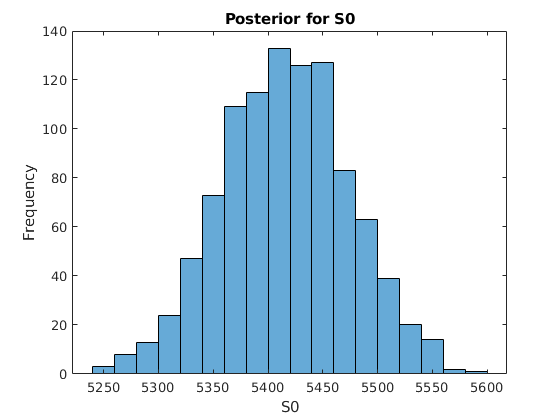
\includegraphics[width=\maxwidth{56.196688409433015em}]{figure_3.png}
\end{center}
\begin{matlabcode}

two_sigma_range_S0_high = mean(bootstrap_samples(1,:)) + 2*std(bootstrap_samples(1,:))
\end{matlabcode}
\begin{matlaboutput}
two_sigma_range_S0_high = 
   5.5323e+03

\end{matlaboutput}
\begin{matlabcode}
two_sigma_range_S0_low = mean(bootstrap_samples(1,:)) - 2*std(bootstrap_samples(1,:))
\end{matlabcode}
\begin{matlaboutput}
two_sigma_range_S0_low = 
   5.2996e+03

\end{matlaboutput}
\begin{matlabcode}

ninety_five_percent_range_S0_high = bootstrap_samples_sorted(1, ceil(length(bootstrap_samples)*(1-0.025)))
\end{matlabcode}
\begin{matlaboutput}
ninety_five_percent_range_S0_high = 
   5.5272e+03

\end{matlaboutput}
\begin{matlabcode}
ninety_five_percent_range_S0_low = bootstrap_samples_sorted(1, ceil(length(bootstrap_samples)*0.025))
\end{matlabcode}
\begin{matlaboutput}
ninety_five_percent_range_S0_low = 
   5.3002e+03

\end{matlaboutput}
\begin{matlabcode}

figure;
histogram(bootstrap_samples(2, :));
xlabel('d');
ylabel('Frequency');
title('Posterior for d');
\end{matlabcode}
\begin{center}
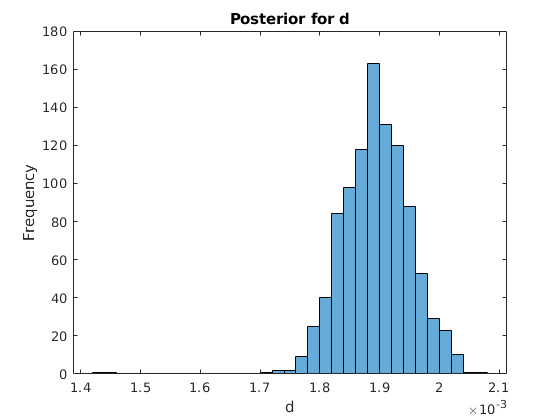
\includegraphics[width=\maxwidth{56.196688409433015em}]{figure_4.png}
\end{center}
\begin{matlabcode}

two_sigma_range_d_high = mean(bootstrap_samples(2,:)) + 2*std(bootstrap_samples(2,:))
\end{matlabcode}
\begin{matlaboutput}
two_sigma_range_d_high = 
   2.0116e-03

\end{matlaboutput}
\begin{matlabcode}
two_sigma_range_d_low = mean(bootstrap_samples(2,:)) - 2*std(bootstrap_samples(2,:))
\end{matlabcode}
\begin{matlaboutput}
two_sigma_range_d_low = 
   1.7782e-03

\end{matlaboutput}
\begin{matlabcode}

ninety_five_percent_range_d_high = bootstrap_samples_sorted(2, ceil(length(bootstrap_samples)*(1-0.025)))
\end{matlabcode}
\begin{matlaboutput}
ninety_five_percent_range_d_high = 
   2.0075e-03

\end{matlaboutput}
\begin{matlabcode}
ninety_five_percent_range_d_low = bootstrap_samples_sorted(2, ceil(length(bootstrap_samples)*0.025))
\end{matlabcode}
\begin{matlaboutput}
ninety_five_percent_range_d_low = 
   1.7897e-03

\end{matlaboutput}
\begin{matlabcode}

figure;
histogram(bootstrap_samples(3, :));
xlabel('f');
ylabel('Frequency');
title('Posterior for f');
\end{matlabcode}
\begin{center}
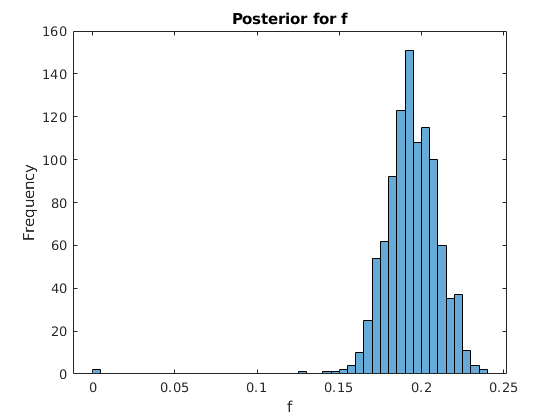
\includegraphics[width=\maxwidth{56.196688409433015em}]{figure_5.png}
\end{center}
\begin{matlabcode}

two_sigma_range_f_high = mean(bootstrap_samples(3,:)) + 2*std(bootstrap_samples(3,:))
\end{matlabcode}
\begin{matlaboutput}
two_sigma_range_f_high = 
   2.2886e-01

\end{matlaboutput}
\begin{matlabcode}
two_sigma_range_f_low = mean(bootstrap_samples(3,:)) - 2*std(bootstrap_samples(3,:))
\end{matlabcode}
\begin{matlaboutput}
two_sigma_range_f_low = 
   1.5971e-01

\end{matlaboutput}
\begin{matlabcode}

ninety_five_percent_range_f_high = bootstrap_samples_sorted(3, ceil(length(bootstrap_samples)*(1-0.025)))
\end{matlabcode}
\begin{matlaboutput}
ninety_five_percent_range_f_high = 
   2.2356e-01

\end{matlaboutput}
\begin{matlabcode}
ninety_five_percent_range_f_low = bootstrap_samples_sorted(3, ceil(length(bootstrap_samples)*0.025))
\end{matlabcode}
\begin{matlaboutput}
ninety_five_percent_range_f_low = 
   1.6574e-01

\end{matlaboutput}


\matlabheadingthree{\textbf{Q1.2.2 - Using Markov Chain Monte-Carlo (MCMC) to provide another estimate of 2-sigma range and 95\% range for paramters.}}


\begin{matlabcode}
% Select a voxel
Avox = dwis(:, 92, 65, 72);

rng(1)
% Generate bootstrap samples - 50 and 700
mcmc_samples = MCMC(Avox, bvals, qhat, 40, 450, 10000);
\end{matlabcode}
\begin{matlaboutput}
Local minimum possible.

fminunc stopped because it cannot decrease the objective function
along the current search direction.

<stopping criteria details>
\end{matlaboutput}


\begin{par}
\begin{flushleft}
Plot parameter values over iterations
\end{flushleft}
\end{par}


\begin{matlabcode}
figure
plot(mcmc_samples(:, 1))
% ylim([4100, 4500])
xlabel('Iterations')
ylabel('S0')
\end{matlabcode}
\begin{center}
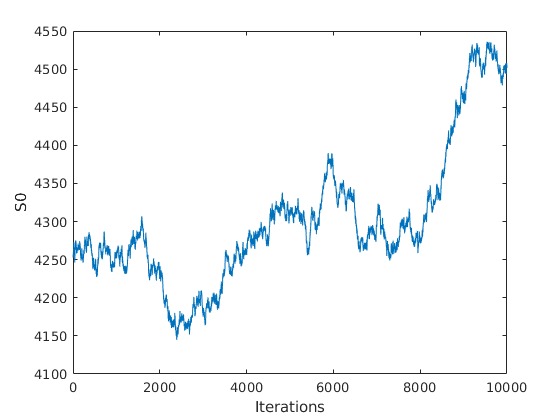
\includegraphics[width=\maxwidth{56.196688409433015em}]{figure_6.png}
\end{center}
\begin{matlabcode}

figure
plot(mcmc_samples(:, 2))
% ylim([0.3, 0.42])
xlabel('Iterations')
ylabel('d')
\end{matlabcode}
\begin{center}
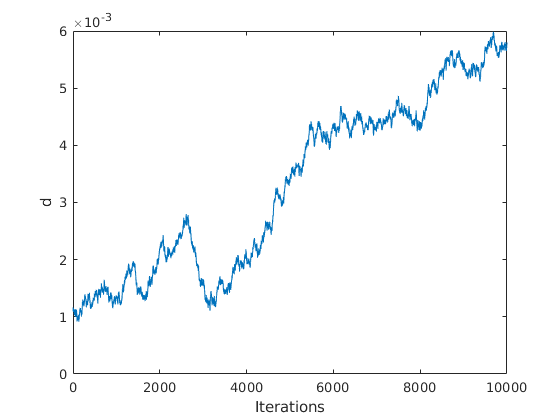
\includegraphics[width=\maxwidth{56.196688409433015em}]{figure_7.png}
\end{center}
\begin{matlabcode}

figure
plot(mcmc_samples(:, 3))
% ylim([1e-03, 1.3e-03])
xlabel('Iterations')
ylabel('f')
\end{matlabcode}
\begin{center}
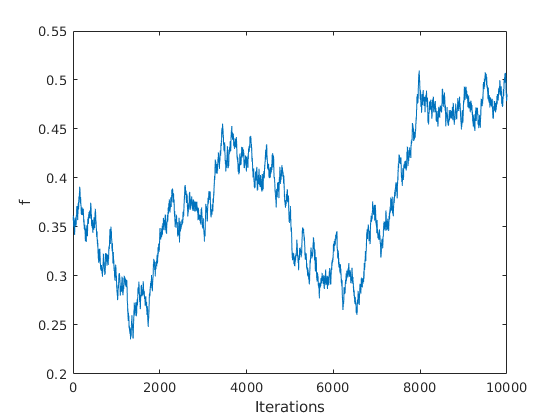
\includegraphics[width=\maxwidth{56.196688409433015em}]{figure_8.png}
\end{center}


\begin{par}
\begin{flushleft}
Plot histograms of parameter samples
\end{flushleft}
\end{par}


\begin{matlabcode}
mcmc_samples_sorted = sort(mcmc_samples, 1, 'ascend');

figure
histogram(mcmc_samples(:, 1))
xlabel('S0');
ylabel('Frequency');
title('Posterior for S0');
\end{matlabcode}
\begin{center}
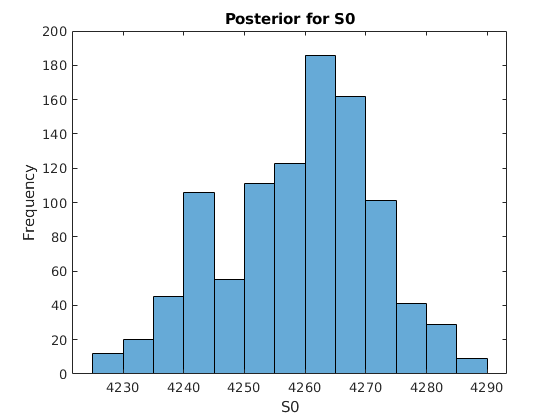
\includegraphics[width=\maxwidth{56.196688409433015em}]{figure_9.png}
\end{center}
\begin{matlabcode}

two_sigma_range_S0_high = mean(mcmc_samples(:, 1)) + 2*std(mcmc_samples(:, 1))
\end{matlabcode}
\begin{matlaboutput}
two_sigma_range_S0_high = 
   4.2839e+03

\end{matlaboutput}
\begin{matlabcode}
two_sigma_range_S0_low = mean(mcmc_samples(:, 1)) - 2*std(mcmc_samples(:, 1))
\end{matlabcode}
\begin{matlaboutput}
two_sigma_range_S0_low = 
   4.2340e+03

\end{matlaboutput}
\begin{matlabcode}

ninety_five_percent_range_S0_high = mcmc_samples_sorted(ceil(length(mcmc_samples)*(1-0.025)), 1)
\end{matlabcode}
\begin{matlaboutput}
ninety_five_percent_range_S0_high = 
   4.2817e+03

\end{matlaboutput}
\begin{matlabcode}
ninety_five_percent_range_S0_low = mcmc_samples_sorted(ceil(length(mcmc_samples)*0.025), 1)
\end{matlabcode}
\begin{matlaboutput}
ninety_five_percent_range_S0_low = 
   4.2330e+03

\end{matlaboutput}
\begin{matlabcode}

figure
histogram(mcmc_samples(:, 2))
xlabel('d');
ylabel('Frequency');
title('Posterior for d');
\end{matlabcode}
\begin{center}
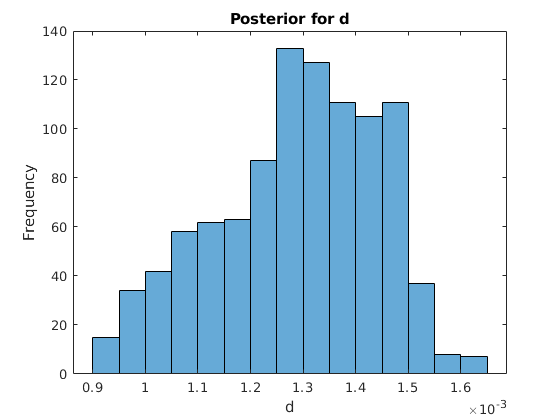
\includegraphics[width=\maxwidth{56.196688409433015em}]{figure_10.png}
\end{center}
\begin{matlabcode}

two_sigma_range_S0_high = mean(mcmc_samples(:, 2)) + 2*std(mcmc_samples(:, 2))
\end{matlabcode}
\begin{matlaboutput}
two_sigma_range_S0_high = 
   1.5969e-03

\end{matlaboutput}
\begin{matlabcode}
two_sigma_range_S0_low = mean(mcmc_samples(:, 2)) - 2*std(mcmc_samples(:, 2))
\end{matlabcode}
\begin{matlaboutput}
two_sigma_range_S0_low = 
   9.7803e-04

\end{matlaboutput}
\begin{matlabcode}

ninety_five_percent_range_S0_high = mcmc_samples_sorted(ceil(length(mcmc_samples)*(1-0.025)), 2)
\end{matlabcode}
\begin{matlaboutput}
ninety_five_percent_range_S0_high = 
   1.5231e-03

\end{matlaboutput}
\begin{matlabcode}
ninety_five_percent_range_S0_low = mcmc_samples_sorted(ceil(length(mcmc_samples)*0.025), 2)
\end{matlabcode}
\begin{matlaboutput}
ninety_five_percent_range_S0_low = 
   9.6327e-04

\end{matlaboutput}
\begin{matlabcode}

figure
histogram(mcmc_samples(:, 3))
xlabel('f');
ylabel('Frequency');
title('Posterior for f');
\end{matlabcode}
\begin{center}
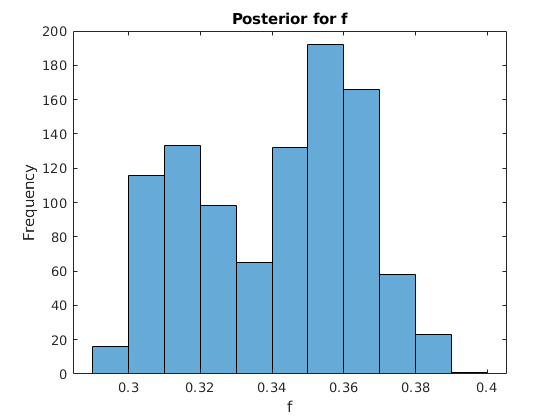
\includegraphics[width=\maxwidth{56.196688409433015em}]{figure_11.png}
\end{center}
\begin{matlabcode}

two_sigma_range_S0_high = mean(mcmc_samples(:, 3)) + 2*std(mcmc_samples(:, 3))
\end{matlabcode}
\begin{matlaboutput}
two_sigma_range_S0_high = 
   3.8749e-01

\end{matlaboutput}
\begin{matlabcode}
two_sigma_range_S0_low = mean(mcmc_samples(:, 3)) - 2*std(mcmc_samples(:, 3))
\end{matlabcode}
\begin{matlaboutput}
two_sigma_range_S0_low = 
   2.9450e-01

\end{matlaboutput}
\begin{matlabcode}

ninety_five_percent_range_S0_high = mcmc_samples_sorted(ceil(length(mcmc_samples)*(1-0.025)), 3)
\end{matlabcode}
\begin{matlaboutput}
ninety_five_percent_range_S0_high = 
   3.7950e-01

\end{matlaboutput}
\begin{matlabcode}
ninety_five_percent_range_S0_low = mcmc_samples_sorted(ceil(length(mcmc_samples)*0.025), 3)
\end{matlabcode}
\begin{matlaboutput}
ninety_five_percent_range_S0_low = 
   3.0168e-01

\end{matlaboutput}


\matlabheading{1.3 Model Selection}


\vspace{1em}
\matlabheadingtwo{Loading Data}


\begin{matlabcode}
% Load the diffusion signal
fid = fopen('data_p1.3-1.4/isbi2015_data_normalised.txt', 'r', 'b');
fgetl(fid); % Read in the header
D = fscanf(fid, '%f', [6, inf])'; % Read in the data
fclose(fid);

% Select the first of the 6 voxels
meas = D(:,1);

% Load the protocol
fid = fopen('data_p1.3-1.4/isbi2015_protocol.txt', 'r', 'b');
fgetl(fid);
A = fscanf(fid, '%f', [7, inf]);
fclose(fid);

% Create the protocol
grad_dirs = A(1:3,:);
G = A(4,:);
delta = A(5,:);
smalldel = A(6,:);
TE = A(7,:);

GAMMA = 2.675987E8;
bvals = ((GAMMA*smalldel.*G).^2).*(delta-smalldel/3);
% convert bvals units from s/m^2 to s/mm^2
bvals = bvals/10^6;
\end{matlabcode}


\matlabheadingtwo{Core Questions: }


\vspace{1em}
\matlabheadingthree{Q1.3.1 - Fit Ball-\&-Stick model from 1.1.3 to the new data.}


\begin{matlabcode}
n_runs = 100;
% Store errors per run here
errors_per_run = zeros(1, n_runs);
min_error = 1e+10;

n = 1;
while n <= n_runs
    % Select a single voxel
    Avox = D(:,1);

    % Define a starting point for the non-linear fit
    startx = [3.5e+00 3e-03 2.5e-01 0 0];
    
    % Add gaussian noise to each of parameters
    startx_noisy(:, 1) = startx(:, 1) + 1e+03*randn;
    startx_noisy(:, 2) = startx(:, 2) + 1e-03*randn;
    % Repeat if the noisy start value isnt within the constraints
    while any(startx_noisy(:, 1:2) < 0)
        startx_noisy(:, 1) = startx(:, 1) + 1e+03*randn;
        startx_noisy(:, 2) = startx(:, 2) + 1e-03*randn;
    end
    startx_noisy(:, 3) = startx(:, 3) + 1e-01*randn;
    % Repeat if the noisy start value isnt within the constraints
    while startx_noisy(:, 3) > 1 || startx_noisy(:, 3) < 0
        startx_noisy(:, 3) = startx(:, 3) + 1e-01*randn;
    end
    startx_noisy(:, 4) = startx(:, 4) + 1e-01*randn;
    startx_noisy(:, 5) = startx(:, 5) + 1e-01*randn;
    
    % Perform inverse transform
    startx_noisy(:, 1:2) = sqrt(startx_noisy(:, 1:2));
    startx_noisy(:, 3) = sqrt(-log(startx_noisy(:, 3)));
    
    % Define various options for the non-linear fitting
    % algorithm.
    h=optimset('MaxFunEvals',20000,...
     'Algorithm','quasi-newton',...
     'TolX',1e-10,...
     'TolFun',1e-10, 'Display', 'off');
    
    % Now run the fitting
    try
        [parameter_hat,RESNORM,EXITFLAG,OUTPUT]=fminunc('BallStickSSD_transformation',startx_noisy,h,Avox,bvals,grad_dirs); 
    catch
        continue
    end
    
%     parameter_hat(:, 1) = parameter_hat(:, 1)^2;
%     parameter_hat(:, 2) = parameter_hat(:, 2)^2;
%     parameter_hat(:, 3) = exp(-parameter_hat(:, 3)^2);
   
    % Store
    errors_per_run(:, n) = RESNORM;
    
    % Save parameters if they have the smallest minimum
    if RESNORM < min_error
        min_error = RESNORM;
        best_params_BS = parameter_hat;
    end
    
    n = n + 1;
end
\end{matlabcode}


\begin{matlabcode}
figure
plot(n_runs)
hold on;
plot(errors_per_run)
xlabel('Iterations')
ylabel('Error')
title('Errors on every iteration')
\end{matlabcode}
\begin{center}
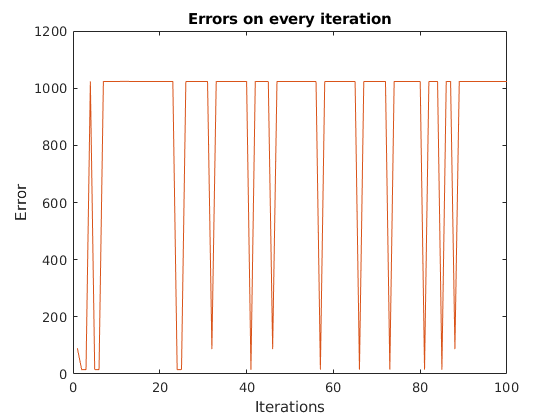
\includegraphics[width=\maxwidth{56.196688409433015em}]{figure_12.png}
\end{center}


\begin{matlabcode}
% Find proportion of trials with smallest value of RESNORM
min_error
\end{matlabcode}
\begin{matlaboutput}
min_error = 
   1.5106e+01

\end{matlaboutput}
\begin{matlabcode}
count = 0;
tolerance = 0.1;
for n=1:n_runs
    if (errors_per_run(n) - min_error <= tolerance)
        count = count + 1;
    end
end

best_params_BS
\end{matlabcode}
\begin{matlaboutput}
best_params_BS = 1x6    
   1.0099e+00   1.4321e-03   5.7493e-01  -1.5447e+00  -8.2863e-02   1.0832e-01

\end{matlaboutput}
\begin{matlabcode}

proportion = count / n_runs
\end{matlabcode}
\begin{matlaboutput}
proportion = 
   1.2000e-01

\end{matlaboutput}
\begin{matlabcode}

% proportion = p(the run will find a global min) = p
% p(atleast 1 global min in n runs) = 1 - p(no global min in N runs)
% 0.95 = 1 - nC0*p^0*(1-p)^n
n_runs = log(0.05)/log(1-proportion)
\end{matlabcode}
\begin{matlaboutput}
n_runs = 
   2.3435e+01

\end{matlaboutput}


\matlabheadingthree{Q1.3.2 - Adapt code further to fit various different models.}


\begin{par}
\begin{flushleft}
Implement Diffusion Tensor Model
\end{flushleft}
\end{par}


\begin{matlabcode}
% Select a single voxel
Avox = D(:, 1);

% Create the design matrix
G = [ones(1, length(Avox)); -bvals.*grad_dirs(1, :).^2; -2*bvals.*grad_dirs(1,:).*grad_dirs(2,:); -2*bvals.*grad_dirs(1,:).*grad_dirs(3,:); -bvals.*grad_dirs(2,:).^2; -2*bvals.*grad_dirs(2,:).*grad_dirs(3,:); -bvals.*grad_dirs(3,:).^2]';

% Compute parameter vector x
x = G\log(Avox);

% Compute error 
S = G*x; 
error = sum((Avox - S).^2)
\end{matlabcode}
\begin{matlaboutput}
error = 
   1.0507e+04

\end{matlaboutput}


\begin{par}
\begin{flushleft}
Implement zeppelin-and-stick model
\end{flushleft}
\end{par}


\begin{matlabcode}
n_runs = 10;
% Store errors per run here
errors_per_run = zeros(1, n_runs);
min_error = 1e+10;

n = 1;
while n <= n_runs
    % Select a single voxel
    Avox = D(:,1);

    % Define a starting point for the non-linear fit
    startx = [3.5e+00 3e-03 2.5e-01 3e-03 0 0];
    
    % Add gaussian noise to each of parameters
    startx_noisy(:, 1) = startx(:, 1) + 1e+03*randn;
    startx_noisy(:, 2) = startx(:, 2) + 1e-03*randn;
    startx_noisy(:, 4) = startx(:, 4) + randn;
    % Repeat if the noisy start value isnt within the constraints
    while any(startx_noisy(:, [1:2, 4]) < 0)
        startx_noisy(:, 1) = startx(:, 1) + 1e+03*randn;
        startx_noisy(:, 2) = startx(:, 2) + 1e-03*randn;
        startx_noisy(:, 4) = startx(:, 4) + randn;
    end
    startx_noisy(:, 3) = startx(:, 3) + 1e-01*randn;
    % Repeat if the noisy start value isnt within the constraints
    while startx_noisy(:, 3) > 1 || startx_noisy(:, 3) < 0
        startx_noisy(:, 3) = startx(:, 3) + 1e-01*randn;
    end
    startx_noisy(:, 5) = startx(:, 5) + 1e-01*randn;
    startx_noisy(:, 6) = startx(:, 6) + 1e-01*randn;
    
    % Perform inverse transformation on first three parameters
    startx_noisy(:, [1:2]) = sqrt(startx_noisy(:, [1:2]));
    startx_noisy(:, 3) = sqrt(-log(startx_noisy(:, 3)));
    startx_noisy(:, 4) = sqrt(startx_noisy(:, 4)/2);
    
    % Define various options for the non-linear fitting
    % algorithm.
    h=optimset('MaxFunEvals',20000,...
     'Algorithm','quasi-newton',...
     'TolX',1e-10,...
     'TolFun',1e-10, 'Display', 'off');
    
    % Now run the fitting
    [parameter_hat,RESNORM,EXITFLAG,OUTPUT]=fminunc('ZeppelinStickSSD',startx_noisy,h,Avox,bvals,grad_dirs);
    
%     parameter_hat(:, 1) = parameter_hat(:, 1)^2;
%     parameter_hat(:, 2) = parameter_hat(:, 2)^2;
%     parameter_hat(:, 3) = exp(-parameter_hat(:, 3)^2);
%     parameter_hat(:, 4) = 2*parameter_hat(:, 4)^2;
   
    % Store
    errors_per_run(:, n) = RESNORM;
    
    % Save parameters if they have the smallest minimum
    if RESNORM < min_error
        min_error = RESNORM;
        best_params_ZS = parameter_hat;
    end
    
    n = n + 1;
end

best_params_ZS
\end{matlabcode}
\begin{matlaboutput}
best_params_ZS = 1x6    
   9.9148e-01   4.0135e-02   9.1189e-01   2.1624e-02  -4.6854e+00  -9.2742e-02

\end{matlaboutput}
\begin{matlabcode}

% Find proportion of trials with smallest value of RESNORM
min_error
\end{matlabcode}
\begin{matlaboutput}
min_error = 
   1.0817e+01

\end{matlaboutput}
\begin{matlabcode}
count = 0;
tolerance = 0.1;
for n=1:n_runs
    if (errors_per_run(n) - min_error <= tolerance)
        count = count + 1;
    end
end

proportion = count / n_runs
\end{matlabcode}
\begin{matlaboutput}
proportion = 
   5.0000e-01

\end{matlaboutput}
\begin{matlabcode}

% proportion = p(the run will find a global min) = p
% p(atleast 1 global min in n runs) = 1 - p(no global min in N runs)
% 0.95 = 1 - nC0*p^0*(1-p)^n
n_runs = log(0.05)/log(1-proportion)
\end{matlabcode}
\begin{matlaboutput}
n_runs = 
   4.3219e+00

\end{matlaboutput}


\begin{par}
\begin{flushleft}
Implement zeppelin-and-stick with tortuousity
\end{flushleft}
\end{par}


\begin{matlabcode}
n_runs = 100;
% Store errors per run here
errors_per_run = zeros(1, n_runs);
min_error = 1e+10;

n = 1;
while n <= n_runs
    % Select a single voxel
    Avox = D(:,1);

    % Define a starting point for the non-linear fit
    startx = [3.5e+00 3e-03 2.5e-01 0 0];
    
    % Add gaussian noise to each of parameters
    startx_noisy(:, 1) = startx(:, 1) + 1e+03*randn;
    startx_noisy(:, 2) = startx(:, 2) + 1e-03*randn;
    % Repeat if the noisy start value isnt within the constraints
    while any(startx_noisy(:, 1:2) < 0)
        startx_noisy(:, 1) = startx(:, 1) + 1e+03*randn;
        startx_noisy(:, 2) = startx(:, 2) + 1e-03*randn;
    end
    startx_noisy(:, 3) = startx(:, 3) + 1e-01*randn;
    % Repeat if the noisy start value isnt within the constraints
    while startx_noisy(:, 3) > 1 || startx_noisy(:, 3) < 0
        startx_noisy(:, 3) = startx(:, 3) + 1e-01*randn;
    end
    startx_noisy(:, 4) = startx(:, 4) + 1e-01*randn;
    startx_noisy(:, 5) = startx(:, 5) + 1e-01*randn;
    
    % Perform inverse transformation on first three parameters
    startx_noisy(:, 1:2) = sqrt(startx_noisy(:, 1:2));
    startx_noisy(:, 3) = sqrt(-log(startx_noisy(:, 3)));
    
    % Define various options for the non-linear fitting
    % algorithm.
    h=optimset('MaxFunEvals',20000,...
     'Algorithm','quasi-newton',...
     'TolX',1e-10,...
     'TolFun',1e-10, 'Display', 'off');
    
    % Now run the fitting
    try
        [parameter_hat,RESNORM,EXITFLAG,OUTPUT]=fminunc('ZeppelinStickTortuositySSD',startx_noisy,h,Avox,bvals,grad_dirs); 
    catch
        continue
    end
    
%     parameter_hat(:, 1) = parameter_hat(:, 1)^2;
%     parameter_hat(:, 2) = parameter_hat(:, 2)^2;
%     parameter_hat(:, 3) = exp(-parameter_hat(:, 3)^2);
   
    % Store
    errors_per_run(:, n) = RESNORM;
    
    % Save parameters if they have the smallest minimum
    if RESNORM < min_error
        min_error = RESNORM;
        best_params_ZST = parameter_hat;
    end
    
    n = n + 1;
end

best_params_ZST
\end{matlabcode}
\begin{matlaboutput}
best_params_ZST = 1x6    
   9.9566e-01  -3.9116e-02  -8.1203e-01  -1.5442e+00  -8.7052e-02   4.9176e-02

\end{matlaboutput}
\begin{matlabcode}

% Find proportion of trials with smallest value of RESNORM
min_error
\end{matlabcode}
\begin{matlaboutput}
min_error = 
   1.1605e+01

\end{matlaboutput}
\begin{matlabcode}
count = 0;
tolerance = 0.1;
for n=1:n_runs
    if (errors_per_run(n) - min_error <= tolerance)
        count = count + 1;
    end
end

proportion = count / n_runs
\end{matlabcode}
\begin{matlaboutput}
proportion = 
   1.3000e-01

\end{matlaboutput}
\begin{matlabcode}

% proportion = p(the run will find a global min) = p
% p(atleast 1 global min in n runs) = 1 - p(no global min in N runs)
% 0.95 = 1 - nC0*p^0*(1-p)^n
n_runs = log(0.05)/log(1-proportion)
\end{matlabcode}
\begin{matlaboutput}
n_runs = 
   2.1511e+01

\end{matlaboutput}


\matlabheadingthree{Q1.3.3 - Compute AIC and BIC for the 3 models.}


\begin{matlabcode}
% Store number of parameters in each model
N_BS = 5;
N_ZS = 6;
N_ZST = 5;

% store number of values in voxel
K = length(Avox);

% compute SSD for each model
SSD_BS = BallStickSSD_transformation(best_params_BS, Avox, bvals, grad_dirs);
SSD_ZS = ZeppelinStickSSD(best_params_ZS, Avox, bvals, grad_dirs);
SSD_ZST = ZeppelinStickTortuositySSD(best_params_ZST, Avox, bvals, grad_dirs);

% compute sigma^2 for each model
sigma_BS = (1/K)*SSD_BS;
sigma_ZS = (1/K)*SSD_ZS;
sigma_ZST = (1/K)*SSD_ZST;

% compute logL for each model
logL_BS = (-K/2)*(log(2*pi) + log(sigma_BS) + 1);
logL_ZS = (-K/2)*(log(2*pi) + log(sigma_ZS) + 1);
logL_ZST = (-K/2)*(log(2*pi) + log(sigma_ZST) + 1);

% Compute AIC score
AIC_BS = 2*(N_BS+1) + K*log((1/K)*SSD_BS)
\end{matlabcode}
\begin{matlaboutput}
AIC_BS = 
  -1.9771e+04

\end{matlaboutput}
\begin{matlabcode}
AIC_ZS = 2*(N_ZS+1) + K*log((1/K)*SSD_ZS)
\end{matlabcode}
\begin{matlaboutput}
AIC_ZS = 
  -2.0975e+04

\end{matlaboutput}
\begin{matlabcode}
AIC_ZST = 2*(N_ZST+1) + K*log((1/K)*SSD_ZST)
\end{matlabcode}
\begin{matlaboutput}
AIC_ZST = 
  -2.0723e+04

\end{matlaboutput}
\begin{matlabcode}

% Compute BIC score
BIC_BS = N_BS*log(K) - 2*logL_BS
\end{matlabcode}
\begin{matlaboutput}
BIC_BS = 
  -9.4831e+03

\end{matlaboutput}
\begin{matlabcode}
BIC_ZS = N_ZS*log(K) - 2*logL_ZS
\end{matlabcode}
\begin{matlaboutput}
BIC_ZS = 
  -1.0690e+04

\end{matlaboutput}
\begin{matlabcode}
BIC_ZST = N_ZST*log(K) - 2*logL_ZST
\end{matlabcode}
\begin{matlaboutput}
BIC_ZST = 
  -1.0444e+04

\end{matlaboutput}

\end{document}
